
\documentclass[10pt]{article}
\usepackage[a4paper,landscape,top=1.6cm,bottom=1.6cm,left=1.8cm,right=1.8cm]{geometry}
\usepackage[utf8]{inputenc}
\usepackage[T1]{fontenc}
\usepackage{lmodern}
\usepackage{microtype}
\usepackage{amsmath,amssymb}
\usepackage{xcolor}
\usepackage[most,breakable]{tcolorbox}
\usepackage{multicol}
\usepackage{booktabs,tabularx,longtable,array,colortbl}
\usepackage{fancyhdr}
\usepackage{enumitem}
\usepackage{lastpage}
\usepackage[hidelinks]{hyperref}
\usepackage{tikz}
\usetikzlibrary{arrows.meta,positioning,calc}
\usepackage{graphicx}

\definecolor{TealBg}{HTML}{E0F2F1}
\definecolor{NavyBg}{HTML}{E8EEFF}

\definecolor{Navy}{HTML}{0D2B6B}
\definecolor{Sky}{HTML}{1976D2}
\definecolor{Teal}{HTML}{00695C}
\definecolor{FGreen}{HTML}{2E7D32}
\definecolor{Amber}{HTML}{E65100}
\definecolor{DRed}{HTML}{B71C1C}
\definecolor{Purple}{HTML}{6A1B9A}
\definecolor{Indigo}{HTML}{303F9F}
\definecolor{LBg}{HTML}{F5F7FA}
\definecolor{BBg}{HTML}{E3F2FD}
\definecolor{GBg}{HTML}{E8F5E9}
\definecolor{RBg}{HTML}{FFEBEE}
\definecolor{ABg}{HTML}{FFF8E1}
\definecolor{IBg}{HTML}{E8EAF6}
\definecolor{TabOdd}{HTML}{EEF2F7}
\definecolor{TGcol}{HTML}{E65100}
\definecolor{QGcol}{HTML}{1565C0}
\definecolor{FGcol}{HTML}{2E7D32}

\tcbuselibrary{skins,breakable}
\tcbset{
  mybox/.style 2 args={
    enhanced, arc=3pt, boxrule=0.7pt,
    fonttitle=\bfseries\small\color{white},
    colbacktitle=#1, colframe=#1, colback=#2,
    lefttitle=5pt, toptitle=3pt, bottomtitle=3pt,
    top=5pt, bottom=5pt, left=6pt, right=6pt,
    before skip=5pt, after skip=5pt, breakable
  }
}
\newcommand{\navybox}[2]{\begin{tcolorbox}[mybox={Navy}{LBg},title={#1}]#2\end{tcolorbox}}
\newcommand{\skybox}[2]{\begin{tcolorbox}[mybox={Sky}{BBg},title={#1}]#2\end{tcolorbox}}
\newcommand{\tealbox}[2]{\begin{tcolorbox}[mybox={Teal}{LBg},title={#1}]#2\end{tcolorbox}}
\newcommand{\greenbox}[2]{\begin{tcolorbox}[mybox={FGreen}{GBg},title={#1}]#2\end{tcolorbox}}
\newcommand{\amberbox}[2]{\begin{tcolorbox}[mybox={Amber}{ABg},title={#1}]#2\end{tcolorbox}}
\newcommand{\redbox}[2]{\begin{tcolorbox}[mybox={DRed}{RBg},title={#1}]#2\end{tcolorbox}}
\newcommand{\purplebox}[2]{\begin{tcolorbox}[mybox={Purple}{LBg},title={#1}]#2\end{tcolorbox}}
\newcommand{\indigobox}[2]{\begin{tcolorbox}[mybox={Indigo}{IBg},title={#1}]#2\end{tcolorbox}}

\newcommand{\pagehead}[2]{%
  \begin{tcolorbox}[enhanced,arc=0pt,outer arc=0pt,boxrule=0pt,
    colback=Navy,colframe=Navy,
    top=5pt,bottom=5pt,left=8pt,right=8pt,
    before skip=0pt,after skip=10pt]
  {\color{white}\large\bfseries #1}%
  \ifx\relax#2\relax\else\\[1pt]{\color{blue!30!white}\small #2}\fi
  \hfill{\color{blue!20!white}\footnotesize Synthetic Financial Time Series $\cdot$ UPC}
  \end{tcolorbox}}

%% audit-row box (used in Extended Data)
\newcommand{\auditrow}[5]{%
  \begin{tcolorbox}[mybox={#2}{#3},
    title={\textbf{[#1]}\quad #4},
    before skip=4pt, after skip=4pt, breakable]
  \small #5
  \end{tcolorbox}}

\pagestyle{fancy}\fancyhf{}\renewcommand{\headrulewidth}{0pt}
\fancyfoot[C]{\small\color{gray!70}
  Page~\thepage\ of~\pageref{LastPage}\quad$\cdot$\quad
  Synthetic Financial Time Series --- GAN Benchmark\quad$\cdot$\quad UPC / BSE}

\newcommand{\tcite}[1]{%
  \hyperlink{R:#1}{\textsuperscript{\scriptsize\textbf{[#1]}}}}

\setlength{\parindent}{0pt}\setlength{\parskip}{4pt}\setlength{\columnsep}{14pt}
\setlist[itemize]{noitemsep,topsep=2pt,leftmargin=14pt,label=\textbullet}
\setlist[enumerate]{noitemsep,topsep=2pt,leftmargin=16pt}
\newcommand{\E}{\mathbb{E}}
\newcommand{\norm}[1]{\left\|#1\right\|}

%% ═══════════════════════════════════════════════════════════════════════════════
\begin{document}

%% ─── Page 1: Title ───────────────────────────────────────────────────────────
\thispagestyle{empty}
\pagecolor{Navy}\color{white}

\vspace*{2.0cm}
\begin{center}
{\fontsize{26}{32}\selectfont\bfseries Synthetic Financial Time Series Generation\par}
\vspace{0.4cm}
{\Large Five Generators, Two Families:\quad GAN\ \ $\cdot$\ \ Econometric\par}
\vspace{0.2cm}
{\large BRICS Emerging Market Indices\par}
\vspace{0.7cm}
\textcolor{blue!40!white}{\rule{0.65\textwidth}{0.5pt}}
\vspace{0.7cm}

\begin{tabular}{r@{\hspace{10pt}}l}
  \textbf{Format}        & Single technical document --- Results $\cdot$ Discussion $\cdot$ Methods $\cdot$ Extended Data \\[4pt]
  \textbf{Collaboration} & Universitat Polit\`{e}cnica de Catalunya (UPC) \\[4pt]
  \textbf{Document type} & Research draft --- prepared for Quantitative Finance / ACM ICAIF \\[4pt]
  \textbf{Gradient-trained} & TimeGAN (GRU) $\cdot$ QuantGAN (TCN-WGAN-GP) $\cdot$ CNN-WGAN-GP (CNN deconvolution) \\[4pt]
  \textbf{Econometric}   & GARCH(1,1)-$t$ $\cdot$ GJR-GARCH(1,1)-$t$ \\[4pt]
  \textbf{Markets}       & BOVESPA $\cdot$ FTSE JSE $\cdot$ MOEX $\cdot$ NIFTY50 $\cdot$ SHANGHAI \\[4pt]
  \textbf{Generated}     & 2026-09-10 \\
\end{tabular}
\end{center}
\clearpage\pagecolor{white}\color{black}

%% ─── Provenance: which run this PDF was built from ─────────────────────────
\begin{tcolorbox}[enhanced,arc=3pt,boxrule=0.8pt,
  colframe=Navy,colback=LBg,left=8pt,right=8pt,top=5pt,bottom=5pt]
\small\textbf{Provenance} --- every number in this report is read from the run below, not hand-typed.
\begin{tabular}{@{}ll@{}}
Generated & 2026-09-08T22:22:54 (git \texttt{7352a023f8}) \\
Seeds & 42, 43, 44 \\
Markets & BOVESPA, FTSE, MOEX, NIFTY50, SHANGHAI \\
Walk-forward folds & 5 \\
Generator updates & 9,000 \\
Software & Python 3.12.3 $\cdot$ PyTorch 2.13.0+cu130 \\
CUDA & yes (NVIDIA GeForce RTX 4090) \\
Platform & Linux-6.8.0-138-generic-x86\_64-with-glibc2.39\\
\end{tabular}
\end{tcolorbox}

%% ─── Abstract + opening ─────────────────────────────────────────────────────
\begin{tcolorbox}[enhanced,arc=4pt,boxrule=1pt,colframe=Navy,colback=LBg,
  top=6pt,bottom=6pt,left=8pt,right=8pt,before skip=2pt,after skip=8pt,
  title={\bfseries Abstract}]
\small
We benchmark five generators of synthetic daily equity returns on five BRICS emerging-market indices, spanning two families: three gradient-trained GANs --- TimeGAN (GRU autoencoder), QuantGAN (causal dilated TCN) and CNN-WGAN-GP (CNN deconvolution), all at an enforced parity of 9,000 generator updates --- and two econometric baselines, GARCH(1,1)-$t$ and GJR-GARCH(1,1)-$t$, fitted by maximum likelihood. Evaluation uses a 14-metric ranked suite split into seven permutation-invariant fidelity metrics and seven ordering-sensitive temporal metrics, with walk-forward temporal validation over 5 folds per market and a shuffled-real control that is scored but excluded from rank competition. The headline result is not a GAN. A 6-parameter GJR-GARCH model, fitted in 0.017\,s, attains the best composite rank (2.543) against a 276,481-parameter QuantGAN trained for 465\,s per market-seed. The split is systematic rather than incidental: the deep models lead on fidelity, which measures the marginal distribution, and the econometric models lead on temporal dynamics, taking 9 of 15 per-market-seed wins on \texttt{temporal\_rank}. The shuffled control exposes why single-score evaluation fails: 9 of 19 computed metrics are permutation-invariant, and on the two most-cited volatility-clustering metrics the control still outscores several genuine generators. Code, artifacts and evaluation pipelines are released.
\end{tcolorbox}

\begin{multicols}{2}

\small
Generative adversarial networks have been applied to financial time series as a data-augmentation and stress-testing tool, with TimeGAN\tcite{4} and QuantGAN\tcite{5} demonstrating qualitative gains over parametric baselines on stylized-fact reproduction. Published benchmarks in this line share three limitations. They concentrate on developed markets (S\&P~500, DAX). They evaluate with metric suites that are largely permutation-invariant --- unable, by construction, to separate a model with correct temporal dynamics from a reordering of real data. And they compare deep generators only with each other, or with a parametric baseline treated as a formality rather than as a competitor. The CNN-WGAN-GP evaluated here is named for its architecture and is distinct from Fin-GAN (Vuleti\'{c}, Prenzel \& Cucuringu 2024)\tcite{41}, which forecasts and classifies returns with an economics-driven loss; ours is an unconditional generator trained with WGAN-GP and makes no forecasts.

We address all three. We evaluate on five genuine BRICS indices, including MOEX, over a 20-year window; we audit the metric suite with a shuffled-real control and report the audit as a result; and we include two econometric baselines fitted on the same data and scored by the same pipeline, on the same footing as the GANs. The third choice is the one that changes the conclusion.

\textbf{The headline.} Across 5 markets $\times$ 3 seeds, the econometric family takes 8 of 15 per-market-seed composite wins and 9 of 15 temporal wins, and GJR-GARCH finishes first overall. This is not an argument that GANs do not work: FinGAN leads the field on \texttt{fidelity\_rank}, and the gradient family takes 9 of 15 fidelity wins. It is an argument that the property the deep models learn best --- the shape of the marginal distribution --- is the property that is cheapest to reproduce and least useful downstream, and that on the dynamics the 6-parameter GJR-GARCH still holds the field.

\textbf{Contributions.} (1) A five-generator, two-family benchmark on genuine BRICS data with per-market training, enforced generator-update parity within the gradient family, and walk-forward evaluation --- 5 markets $\times$ 3 seeds $\times$ 5 folds, all artifacts released. (2) A shuffled-control audit that counts 9 of 19 metrics as permutation-invariant in this run, and shows that permutation-invariance in practice is a property of the comparison set, not of a metric in isolation. (3) A compute-versus-performance accounting that a benchmark reporting rank alone cannot make. (4) Empirical demotion of both ARCH-LM variants, of \texttt{kurtosis\_diff} and \texttt{skewness\_diff} (population moments that do not exist at the measured tail indices), and of unconditional VaR, each with the measurement that motivated it.

\end{multicols}

\clearpage

%% ─── Results 1: headline ranking + compute ─────────────────────────────────
\pagehead{Results --- Model Ranking Across Two Families}
         {5 markets $\times$ 3 seeds $\times$ 5 walk-forward folds $\cdot$ generator-update parity within the gradient family}

\begin{multicols}{2}

\navybox{Composite Ranking (Table~1)}{%
Ranks are computed among the generators present in \texttt{overall\_performance.csv}; the shuffled control is scored on every metric but excluded from rank competition and reported separately. \texttt{Wins} counts the (market, seed) cells in which a model attains the lowest \texttt{composite\_rank}, out of 15.

\smallskip
\resizebox{\linewidth}{!}{%
\begin{tabular}{@{}llccccr@{}}
\toprule
Model & Family & composite & fidelity & temporal & Wins & Fit (s) \\
\midrule
GJR-GARCH & econometric & \textbf{2.543} & 2.705 & 2.381 & 3\,/\,15 & $<1$ \\
FinGAN & gradient & 2.714 & 2.486 & 2.943 & 2\,/\,15 & 173 \\
QuantGAN & gradient & 2.912 & 3.062 & 2.762 & 5\,/\,15 & 465 \\
GARCH & econometric & 2.950 & 3.138 & 2.762 & 5\,/\,15 & $<1$ \\
TimeGAN & gradient & 3.881 & 3.610 & 4.152 & 0\,/\,15 & 77 \\
\bottomrule
\end{tabular}}

\smallskip
Composite wins: GARCH 5, QuantGAN 5, GJR-GARCH 3, FinGAN 2. The econometric family takes 8 of 15.

Temporal wins: GJR-GARCH 5, GARCH 4, QuantGAN 4, FinGAN 2 --- econometric 9 of 15.

Fidelity wins: FinGAN 6, GJR-GARCH 4, QuantGAN 3, GARCH 2 --- gradient 9 of 15.

\smallskip
The two families separate along the two metric families, and in opposite directions. Deep generators lead on fidelity, which measures how closely the synthetic marginal distribution matches the real one. Econometric models lead on temporal, which measures whether the ordering behaves like a market. The composite is the equal-weighted mean of the two, and on that measure GJR-GARCH finishes first.

\smallskip
\texttt{avg\_rank} is the unweighted mean over all 14 ranked metrics. It is retained for comparability only and is never the selection criterion: an unweighted mean over metrics is won by the shuffled control, because 9 of the 19 computed metrics score a permutation of the real data perfectly by construction. Model selection uses \texttt{composite\_rank}.}

\columnbreak

\redbox{Compute Versus Performance (Table~2)}{%
Nothing in a rank column carries the cost of obtaining it. Parameter counts are the fitted or trainable parameters actually recorded per run; wall-clock is the mean fit or train time for one (market, seed).

\smallskip
\resizebox{\linewidth}{!}{%
\begin{tabular}{@{}llrrrc@{}}
\toprule
Model & Family & Params & Gen.\ updates & Fit (s) & composite \\
\midrule
GJR-GARCH & econometric & 6 & n/a & 0.017 & 2.543 \\
GARCH & econometric & 5 & n/a & 0.018 & 2.950 \\
TimeGAN & gradient & 11,400 & 9,000 & 77.1 & 3.881 \\
FinGAN & gradient & 55,401 & 9,000 & 172.9 & 2.714 \\
QuantGAN & gradient & 276,481 & 9,000 & 464.7 & 2.912 \\
\bottomrule
\end{tabular}}

\smallskip
The best-ranked model in this benchmark, GJR-GARCH, has 6 parameters and is fitted in 0.017\,s. The largest, QuantGAN, has 276,481 --- a factor of 46,080 --- and takes 465\,s, a factor of 27,242 in wall-clock. It ranks below the smaller model on composite, on fidelity and on temporal.

\smallskip
Econometric rows carry \texttt{n/a} in the generator-updates column rather than a number. Maximum-likelihood fitting has no gradient-step analogue, and printing one would invent a quantity the run never produced. The parity assertion that binds the three GANs to a common budget is scoped to the gradient family for the same reason (Methods).

\smallskip
We state the ratio and leave it there. The measurement does not establish that parameter count is wasted in general, that the GANs would not overtake the baselines at a larger budget, or that these architectures are at their best configuration --- no hyperparameter search was run (Discussion). What it does establish is that on this data, at this budget, under this evaluation, the additional capacity did not buy additional rank.}

\end{multicols}

\clearpage

%% ─── Results 2: the shuffled-control audit ─────────────────────────────────
\pagehead{Results --- The Shuffled-Control Audit}
         {What a permutation of the real data scores, and what that does and does not prove}

\begin{multicols}{2}

\skybox{Permutation-Invariance, Counted}{%
The control is the pooled real test series in random order (\texttt{numpy.random.default\_rng(42).permutation}). It has the identical marginal distribution --- same values, same histogram, same moments, same tails --- and no temporal structure whatsoever. It is useless for every application synthetic market data is generated for, and it is scored by the full pipeline alongside every generator.

\smallskip
A metric is counted as permutation-invariant in practice when the control's mean value is negligible against the best real generator's on the same metric. On this run that criterion separates cleanly: every metric it selects has a ratio below 3.4e-05, and the smallest ratio among the metrics it does not select is 0.35. There is nothing in the gap, so the cut is not a judgement call.

\smallskip
\textbf{9 of 19} computed metrics are permutation-invariant:
{\footnotesize\texttt{mean\_diff, std\_diff, skewness\_diff, kurtosis\_diff, wasserstein, energy\_distance, quantile\_mse, tail\_index\_diff, extreme\_events\_diff}}

\smallskip
Under an unweighted mean over all metrics, the control ranks first --- the finding that produced the two-family composite. That is a structural property of any metric defined on the marginal distribution alone, not a quirk of these choices: mean, variance, kurtosis, Wasserstein distance and energy distance all belong to that class. Any evaluation of synthetic financial data built only from distributional metrics cannot distinguish a working generator from a shuffled deck.}

\amberbox{The Harder Finding (Table~3)}{%
The count above is the part that is true by construction, and by itself it is not very interesting: those metrics are permutation-invariant because they are defined to be. The result that matters is what happens on the metrics that are \emph{ordering-sensitive} by construction --- the ones a shuffled deck is supposed to fail.

\smallskip
Mean over all 15 market-seeds. Bold marks the better value; models are bold where they beat the control.

\smallskip
\resizebox{\linewidth}{!}{%
\begin{tabular}{@{}lcccccc@{}}
\toprule
Metric & Control & FinGAN & GARCH & GJR-GARCH & QuantGAN & TimeGAN \\
\midrule
ACF$(r)$ MAE & \textbf{0.0517} & \textbf{0.0512} & \textbf{0.0514} & \textbf{0.0514} & 0.0535 & 0.0685 \\
ACF$(r^2)$ MAE & \textbf{0.0570} & 0.0576 & \textbf{0.0541} & \textbf{0.0544} & 0.0732 & 0.1002 \\
ACF$(|r|)$ MAE & \textbf{0.0730} & \textbf{0.0636} & \textbf{0.0593} & \textbf{0.0610} & 0.0839 & 0.1232 \\
Hurst diff & \textbf{0.0759} & \textbf{0.0381} & \textbf{0.0404} & \textbf{0.0341} & \textbf{0.0410} & 0.0881 \\
\bottomrule
\end{tabular}}

\smallskip
On \textbf{ACF$(r^2)$ MAE} --- the canonical volatility-clustering statistic --- the shuffled control beats \emph{all 3 GANs}. Only GARCH, GJR-GARCH clear it.

On \textbf{ACF$(|r|)$ MAE} the control beats QuantGAN, TimeGAN; FinGAN, GARCH, GJR-GARCH clear it.

On \textbf{ACF$(r)$ MAE} the control beats QuantGAN, TimeGAN, and the models that do clear it do so by 0.0003 to 0.0005 --- margins on the fourth decimal.

On \textbf{Hurst diff} the control beats TimeGAN alone.

\smallskip
A shuffled copy of the real series, carrying no temporal information at all, outperforms state-of-the-art GAN architectures on the metrics those architectures exist to satisfy.}

\columnbreak

\purplebox{What This Does and Does Not License}{%
It is tempting to conclude that these ACF metrics are ``really'' permutation-invariant too, and to move the headline count from 9 to a larger number. We do not, and the reason is the contribution.

\smallskip
\textbf{These metrics are not permutation-invariant.} They are functions of the ordering, and they separate the econometric models from the control on every row of Table~3. A metric that can make that separation is measuring temporal structure. It is doing its job.

\smallskip
\textbf{What fails is the comparison, not the metric.} A metric that separates GARCH from a shuffled deck but does not separate three GANs from it is telling us something about the GANs. Read the other way round, it is weak evidence about the metric.

\smallskip
\textbf{Therefore: permutation-invariance in practice is a property of the comparison set, not of a metric in isolation.} The same metric is discriminating against one model and uninformative against another, in the same run, on the same data. A count of ``how many metrics are permutation-invariant'' is only meaningful once the set of models being compared is fixed --- and reporting one without the other is how a suite comes to look more discriminating than it is.

\smallskip
We keep the headline at 9 of 19: the metrics that are invariant by construction. The ACF results are reported as what they are --- a failure of three generators, on the metrics most often used to claim success --- and \texttt{FIDELITY\_COLS} and \texttt{TEMPORAL\_COLS} are unchanged.

\smallskip
The practical recommendation follows: a shuffled control belongs in every evaluation table for synthetic time series, permanently, in the role a positive control plays in a biology experiment. It costs one permutation and it is the only line in the table that cannot be gamed by learning the marginal.}

\end{multicols}

\clearpage

%% ─── Results 3: walk-forward, tails, failure modes ─────────────────────────
\pagehead{Results --- Walk-Forward Validation and Failure Modes}
         {Discriminative AUC against the empirical null $\cdot$ tail-index dispersion $\cdot$ mode collapse $\cdot$ metric circularity}

\begin{multicols}{2}

\navybox{Discriminative AUC Against the Empirical Null (Table~4)}{%
A logistic classifier on 20-day rolling windows (features: mean, sd, mean-abs, mean-sq) is trained to separate real from synthetic. AUC $=0.5$ would be indistinguishability --- but the null is not exactly $0.5$. Measured over 15 real-vs-real half-splits it is $\mathbf{0.506 \pm 0.084}$, and every AUC below is read against that.

\smallskip
\resizebox{\linewidth}{!}{%
\begin{tabular}{@{}lcccr@{}}
\toprule
Model & AUC (mean $\pm$ sd) & $|$AUC$-0.5|$ & $z$ vs null & Folds \\
\midrule
FinGAN & 0.640 $\pm$ 0.146 & 0.140 & 1.60 & 75 \\
GARCH & 0.699 $\pm$ 0.168 & 0.199 & 2.30 & 75 \\
GJR-GARCH & 0.658 $\pm$ 0.160 & 0.158 & 1.80 & 75 \\
QuantGAN & 0.737 $\pm$ 0.193 & 0.237 & 2.75 & 75 \\
TimeGAN & 0.814 $\pm$ 0.144 & 0.314 & 3.66 & 75 \\
\bottomrule
\end{tabular}}

\smallskip
Measured against that null, 3 of 5 models sit more than 1.96 null sd away (TimeGAN, QuantGAN, GARCH). The remainder (FinGAN, GJR-GARCH) lie within 1.96 null sd on the fold-averaged mean and cannot, on this metric alone, be distinguished from a perfect generator at the 5\% level. 5 of 5 mean AUCs lie above the null mean. Ranking is on $|\text{AUC}-0.5|$, never on the raw value: under an ascending rank on raw AUC an anti-predictive classifier at $0.30$ would outrank an indistinguishable one at $0.50$, which inverts the meaning of the metric.

\smallskip
Cross-validation is not shuffled. The 20-day windows overlap by 19 observations, so \texttt{shuffle=True} places near-duplicates in both train and test; measured, that moves the null from $0.506$ to $0.584$. Unshuffled CV is the correct design here, and the shift is the evidence.}

\amberbox{The Fold-Length Effect --- and Its Confound (Table~5)}{%
Each walk-forward fold retrains from scratch on a longer training segment than the last.

\smallskip
\begin{tabular}{@{}lccc@{}}
\toprule
Fold & Train length & Mean AUC & sd \\
\midrule
0 & 810--837 & 0.818 & 0.156 \\
1 & 1,620--1,669 & 0.694 & 0.141 \\
2 & 2,430--2,501 & 0.743 & 0.148 \\
3 & 3,240--3,333 & 0.635 & 0.189 \\
4 & 4,050--4,165 & 0.658 & 0.169 \\
\bottomrule
\end{tabular}

\smallskip
AUC falls as fold training length grows: 0.818 at fold 0 (training on 810--837 points) against 0.658 at fold 4 (4,050--4,165). The decline is \textbf{not monotonic}: fold(s) 2, 4 rise above the fold before. We report it as a trend, not a monotone relationship, because the folds do not support the stronger claim.

\smallskip
\textbf{The confound is not separated.} Fold index, training-set length and the specific historical period a fold covers all advance together by construction of the walk-forward schedule. A later fold trains on more data \emph{and} on a different market regime. Nothing in this design distinguishes ``more training data helps'' from ``the later period is easier to imitate''. Separating them needs folds at fixed length on rolling windows, which this run does not have. We state the trend and the confound together; the trend alone would be a claim we have not earned.}

\columnbreak

\tealbox{Tail-Index Dispersion (Table~6)}{%
\texttt{tail\_index\_diff} is the ranked heavy-tail metric --- the absolute difference in Hill\tcite{38} $\hat\alpha$ between real and synthetic.

\smallskip
\begin{tabular}{@{}lccc@{}}
\toprule
Model & Mean & sd & Observed range \\
\midrule
FinGAN & 1.242 & 0.908 & 0.006--2.994 \\
GARCH & 1.238 & 1.120 & 0.086--3.785 \\
GJR-GARCH & 1.316 & 0.856 & 0.019--2.385 \\
QuantGAN & 1.098 & 0.908 & 0.013--2.865 \\
TimeGAN & 2.682 & 3.330 & 0.024--9.825 \\
\bottomrule
\end{tabular}

\smallskip
TimeGAN sits at 2.68 against 1.10--1.32 for the other four --- a real and large gap.

\smallskip
\textbf{But the dispersion swamps the comparison.} The spread between model means is 1.58; the largest within-model standard deviation across market-seeds is 3.33, which exceeds it. Every model's observed range overlaps every other model's except TimeGAN's upper reach. Run-to-run and market-to-market variation on this metric is larger than most of the differences between models, so a single-run winner on \texttt{tail\_index\_diff} is not a finding, and none is reported.}

\redbox{TimeGAN: Mode Collapse, Caught by the Guard}{%
The pipeline's post-generation guard checks every generated series and prints a \texttt{[WARNING]} when the lag-1 autocorrelation exceeds $|0.1|$ --- a return series should have almost none, and a high value means a smooth path rather than returns.

\smallskip
In this run the guard fired \textbf{16 times}, all of them TimeGAN (16), and never for any other model. Mean \(|\text{ACF}(1)| = 0.568\), over the range \(-0.622\) to \(0.942\); generated sd 0.0069--0.0191. Read from \texttt{run\_log\_20260908\_222254.log}.

\smallskip
The ranking agrees. TimeGAN is the worst of the five on \textbf{all 7 of 7 temporal metrics}, on 5 of 7 fidelity metrics, and on 15 of the 19 computed metrics overall. It is \emph{not} worst on std\_diff (QuantGAN), skewness\_diff (QuantGAN), quantile\_mse (QuantGAN), arch\_pvalue\_diff (GARCH) --- the model in brackets is worse there --- so ``worst on every metric'' would be an overstatement, and the scope is stated instead.

\smallskip
\textbf{An earlier explanation is withdrawn.} A previous draft attributed this to tanh saturation in the Recovery network. This run's own \texttt{[DIAG]} latent instrumentation does not support that: across 90 latent readings saturation never exceeds 3.1\% against the 50\% threshold the diagnostic exists to detect, and across 90 reconstruction readings output sd never differs from target sd by more than 0.0014, so the autoencoder is functioning. The collapse is real and the mechanism is open.}

\indigobox{Metric Circularity: \texttt{resid\_kurtosis\_diff}}{%
Stated before a referee states it. \texttt{resid\_kurtosis\_diff} fits a GARCH(1,1) to each series, extracts $\varepsilon_t = r_t/\sigma_t$, and compares the excess kurtosis of those residuals. Two of the five generators \emph{are} GARCH models, so they are being scored, in part, by their own model class.

\smallskip
This is not fatal, and the reason is what the metric asks. It does not ask ``does a GARCH fit this series'' --- that would be circular outright. It asks whether the tails remain heavy \emph{after} GARCH has removed what it can explain, which is Cont's stylized fact 7\tcite{7} and a property a GARCH-$t$ generator can fail. The measured values bear this out: the econometric models score GARCH 3.12, GJR-GARCH 3.04, against 2.68--4.02 for the GANs and 0.94 for the shuffled control --- neither scores better than the shuffled control on it.

\smallskip
It remains an advantage of degree, and it is one reason \texttt{composite\_rank} is reported alongside its two components rather than alone --- \texttt{resid\_kurtosis\_diff} is one of seven temporal metrics, and the temporal result does not rest on it. Gaussian QMLE is used for the fit rather than Student-$t$ precisely to avoid the stronger circularity: a $t$ specification absorbs the excess kurtosis by construction and makes the test uninformative for every model.}

\end{multicols}

\clearpage

%% ─── Results 4: downstream utility, ARCH-LM, budget, determinism ───────────
\pagehead{Results --- Downstream Utility, Budget Sensitivity and Reproducibility}
         {TSTR risk models $\cdot$ ARCH-LM regime failure $\cdot$ what the budget choice cost $\cdot$ run-to-run drift}

\begin{multicols}{2}

\navybox{Downstream Utility: Train-Synthetic, Test-Real (Table~7)}{%
Distributional metrics say whether synthetic data \emph{looks} real. This asks whether a practitioner can build a working risk model on it: fit GARCH(1,1) on the synthetic series, filter the fitted parameters over real test returns for one-step-ahead $\sigma_t$, set $\text{VaR}_t = \mu + \sigma_t z_\alpha$, and backtest with Kupiec\tcite{34} and Christoffersen\tcite{35}. Lower QLIKE\tcite{37} is better.

\smallskip
\resizebox{\linewidth}{!}{%
\begin{tabular}{@{}lrrrrrrc@{}}
\toprule
Model & QLIKE med & QLIKE mean & Cov.\ err & Kupiec $p$ & Viol. & $n$ & Fail \\
\midrule
FinGAN & -8.158 & -7.8 & 0.0109 & 0.252 & 27 & 496 & --- \\
GJR-GARCH & -8.130 & -8.1 & 0.0157 & 0.119 & 26 & 496 & --- \\
GARCH & -8.129 & 2,197.9 & 0.0177 & 0.054 & 23 & 496 & 1 \\
QuantGAN & -8.094 & -7.8 & 0.0206 & 0.034 & 21 & 496 & --- \\
TimeGAN & -8.056 & -7.7 & 0.0220 & 0.030 & 24 & 496 & --- \\
CONTROL: shuffled real & -8.005 & 3,388.5 & 0.0077 & 0.422 & 25 & 496 & 3 \\
\bottomrule
\end{tabular}}

\smallskip
\textbf{Median and mean are both shown, and they disagree.} 4 of 90 model-market-seed cells returned a positive QLIKE:

\smallskip
{\footnotesize
\begin{tabular}{@{}llrrrr@{}}
\toprule
Model & Market & Seed & QLIKE & Viol. & $n$ \\
\midrule
GARCH & MOEX & 42 & 33,081 & 256 & 500 \\
CONTROL: shuffled real & FTSE & 42 & 16,975 & 237 & 501 \\
CONTROL: shuffled real & FTSE & 43 & 16,975 & 237 & 501 \\
CONTROL: shuffled real & FTSE & 44 & 16,975 & 237 & 501 \\
\bottomrule
\end{tabular}}

\smallskip
QLIKE averages $\log\sigma_t^2 + r_t^2/\sigma_t^2$ over observations, so a variance forecast near zero on a single observation sends that term toward infinity, and one such cell then dominates any mean taken across cells. \textbf{The mean column is therefore uninformative here:} CONTROL: shuffled real's mean of 3,388.47 against a median of $-$8.01 is an artefact of 3 degenerate cells, not a summary. The cells are reported, not removed --- removing them would change a measured result --- and the median is the column to read.

\smallskip
\textbf{On $n$.} The files are named \texttt{pooled\_downstream\_utility.csv}, but each carries one market's test set: $n$ ranges from 486 to 501 across 15 files, combining to 2,479 across the 5 markets. What is reported above is therefore a summary of 15 per-market backtests, \textbf{not} a single pooled backtest at the combined $n$ --- these artifacts predate the pipeline's pooled computation. The distinction is not cosmetic: the per-market $n$ is below the $n\approx2{,}480$ at which Kupiec power was measured at $\approx99\%$ (it is $\approx56\%$ at $n\approx496$), so the per-market $p$-values above are descriptive, and QLIKE is the primary downstream signal.}

\columnbreak

\amberbox{ARCH-LM: A Regime Failure, Reported as a Result}{%
An 80-replication Monte Carlo (GARCH(1,1), $n=1{,}200$, Gaussian innovations) found \texttt{arch\_pvalue\_diff} identifies the better-fitting model $99\%$ of the time and \texttt{arch\_stat\_diff} $76\%$, the latter with null sd $\approx46.4$ --- two draws from the same process gave LM $56.8$ and $124.8$.

\smallskip
On real BRICS data the pvalue variant saturates completely: real and shuffled series both underflow to $p=0.0$, so $|\Delta p| = 0.000000$ and the metric rates the adversarial control as a perfect match. The stat variant detects the control but is too noisy to rank on.

\smallskip
Neither variant is reliable across both regimes, so both are descriptive-only. ACF-MAE is the primary volatility-clustering ranking signal: continuous, no saturation regime, $88\%$ accuracy in the same Monte Carlo. This is an empirical result about a standard test, not an implementation note.}

\redbox{What the Budget Choice Cost}{%
Budget parity fixes which models are compared fairly. It does not fix \emph{at what budget}, and that choice moves the answer.

\smallskip
At a smoke-test budget of 1{,}000 generator updates, QuantGAN won all five repeat runs on \texttt{composite\_rank} (1.429--1.500), with CNN-WGAN-GP at 1.786--1.893 --- a prior measurement recorded in the repository's standing constraints, not reproducible from this run's artifacts.

\smallskip
At 9,000 generator updates, ordering the 3 gradient-trained models by \texttt{composite\_rank} within this five-model ranking gives FinGAN 8\,/\,15, QuantGAN 6\,/\,15, TimeGAN 1\,/\,15. FinGAN leads.

\smallskip
\textbf{The winner changed.} Ranking at a smoke-test budget did not predict ranking at full budget. This is the budget-parity lesson one level up: even with parity correctly enforced, the budget you evaluate at determines the result.

\smallskip
Most papers in this literature report a single budget without justifying the choice. We report ours --- and state plainly that 9,000 updates is itself a choice whose sensitivity we have only partially characterised. Two points on a budget curve is not a budget curve. A benchmark that reports one point is reporting a result conditional on an unstated hyperparameter.}

\purplebox{Run-to-Run Nondeterminism at Fixed Seed}{%
At fixed seed and identical code, five repeated runs show sharply different stability by architecture. TimeGAN and the shuffled control are bit-identical across all five --- sd $=0$ on every metric, every fold. CNN-WGAN-GP drifts slightly: Wasserstein CV $1.6\%$, walk-forward AUC sd $0.009$. QuantGAN drifts substantially: Wasserstein CV $37\%$, \texttt{tail\_index\_diff} CV $79\%$, raw AUC $0.551$--$0.734$.

\smallskip
This is not a seeding bug. Loss traces agree to four significant figures at epoch~1 and separate by epoch~5, consistent with QuantGAN being the only model combining WGAN-GP's double-backward gradient penalty with dilated convolutions.

\smallskip
\texttt{torch.use\_deterministic\_algorithms(True)} and \texttt{cudnn.deterministic} remain deliberately unset. The consequence is now measured rather than assumed, and that is the justification: \texttt{composite\_rank} is stable across runs, but \texttt{tail\_index\_diff}, \texttt{hurst\_diff} and \texttt{mean\_diff} change their winning model between identical repeat runs. That is why no single-run winner on those metrics appears anywhere in this report.}

\end{multicols}

\clearpage

%% ─── Figures: this run's plots, included by reference ──────────────────────
\pagehead{Figures --- BOVESPA (seed 42)}
         {Seven stacked series rows --- real, five generators, shuffled control --- plus the log-log tail panel}

\clearpage\begin{center}
\includegraphics[width=0.85\linewidth,height=0.78\textheight,keepaspectratio]{thesis_results/production/BOVESPA/seed42/BOVESPA_stylized_facts.png}\end{center}\begin{center}\begin{minipage}{0.88\linewidth}\small\textit{Stylised facts: every series against real daily log returns. The top block is one full-width row per series --- real, each generator, and the shuffled control --- on a single shared y-scale; the x-axis is a common index, not a common time, since real and synthetic are independent unconditional draws and vertical alignment between rows carries no correspondence. The tail panel plots the empirical survival function \$P(|r| > x)\$ on log-log axes: a power-law tail is a straight line there, and its slope is the tail index \$\textbackslash{}alpha\$, so a model whose line runs parallel to the real series matches the tail exponent while one that falls away below it under-produces extremes. Lines and axis are cut at roughly \$1/n\$, because the largest few order statistics are single-point estimates of an extreme probability; the trim affects the drawn line only, never a metric.}\end{minipage}\end{center}\vspace{6pt}

\clearpage\begin{center}
\includegraphics[width=0.85\linewidth,height=0.78\textheight,keepaspectratio]{thesis_results/production/BOVESPA/seed42/BOVESPA_metrics_heatmap.png}\end{center}\begin{center}\begin{minipage}{0.88\linewidth}\small\textit{Normalised metrics heatmap, one column per metric and one row per series. Colour is within-metric normalised, so it compares models on a metric and never metrics with each other.}\end{minipage}\end{center}\vspace{6pt}

\clearpage\begin{center}
\includegraphics[width=0.85\linewidth,height=0.78\textheight,keepaspectratio]{thesis_results/production/BOVESPA/seed42/BOVESPA_rank_comparison.png}\end{center}\begin{center}\begin{minipage}{0.88\linewidth}\small\textit{Average rank across all ranked metrics. Shown for comparability only: avg\textbackslash{}\_rank is not the selection criterion, because an unweighted mean over metrics is won by the shuffled control. Model selection uses composite\textbackslash{}\_rank.}\end{minipage}\end{center}\vspace{6pt}

\clearpage

%% ─── Discussion ────────────────────────────────────────────────────────────
\pagehead{Discussion}
         {What the two-family result means $\cdot$ the audit as a contribution $\cdot$ limitations $\cdot$ future work}

\begin{multicols}{2}

\navybox{A 6-Parameter Model Wins, and Why That Is the Interesting Part}{%
The result is not that deep generative models fail. FinGAN leads the field on \texttt{fidelity\_rank} and the gradient family takes 9 of 15 fidelity wins; these models reproduce the marginal distribution of BRICS returns well, including tails that defeat a Gaussian by orders of magnitude.

The result is that reproducing the marginal is not the hard part, and it is not the part that transfers. On \texttt{temporal\_rank} --- volatility clustering, long memory, conditional heavy tails, indistinguishability --- the econometric family takes 9 of 15, and GJR-GARCH finishes first overall on the equal-weighted composite.

Two readings are available and the data does not settle between them. Either the GAN architectures have not been given enough budget, capacity or tuning to reach their potential here --- no hyperparameter search was run, and the budget-sensitivity result shows the budget matters --- or conditional heteroskedasticity with a leverage term is simply a very good model of daily equity returns, and a general-purpose sequence generator learning it from scratch on $\approx$4{,}000 observations per market is at a structural disadvantage. Both are consistent with what we measured. What is not consistent with what we measured is a benchmark that omits the parametric baseline and reports the best GAN as the state of the art.

\smallskip
This is why the econometric arm was added. A benchmark of GANs against GANs answers ``which GAN'', and produces a winner regardless of whether any entrant is useful.}

\skybox{The Audit as a Methodological Contribution}{%
The shuffled control is the cheapest useful thing in this pipeline: one permutation of the test set, scored by the same code as everything else.

It establishes two things. First, 9 of 19 computed metrics score it perfectly by construction, so any composite that mixes families without balancing them is won by a sequence with no temporal content. The fix --- taxonomise metrics by invariance, weight families rather than metrics, exclude the control from rank competition --- needs no additional computation.

Second, and less comfortably: on the ordering-sensitive metrics the control still outperforms genuine GAN generators. That is not a metric failure. It is a measurement of the generators, made possible only because a control was present to make it against.

\smallskip
The general form of the caveat is the part we would ask others to adopt. \textbf{Whether a metric discriminates is a joint property of the metric and the model set.} The same statistic separates GARCH from a shuffled deck and fails to separate three GANs from it, in one run, on one dataset. Reporting a suite's discriminating power without naming the models it was measured against overstates it.}

\columnbreak

\redbox{Limitations}{%
\textbf{No hyperparameter search.} All three GAN architectures use reference-implementation defaults from their original papers. No search over learning rate, hidden dimension or noise dimension has been run (Bergstra \& Bengio 2012\tcite{12} would be the protocol). The econometric baselines have no comparable free parameters, so this asymmetry favours the baselines and is stated as such. It is the largest single caveat on the headline result.

\textbf{One budget, partially characterised.} See Results: the winner among the GANs changes between a smoke-test budget and 9,000 updates. Two points do not characterise a curve.

\textbf{No diffusion baseline.} Takahashi \& Mizuno (2025)\tcite{29} report diffusion-based generators outperforming GANs on several stylized-fact metrics. This benchmark does not include one. Reviewers will ask; the answer is not yet.

\textbf{Fold confound unseparated.} Fold index, training length and historical period advance together (Results, Table~5).

\textbf{Downstream utility per market, not pooled.} These artifacts predate the pipeline's pooled computation (Methods), and 4 of 90 cells returned a degenerate QLIKE, reported with the median beside the mean.

\textbf{Crisis regimes remain few.} Twenty years resolves the estimator problem --- Hill sd falls from $\approx$0.52 at $n=995$ to $\approx$0.035 at $n\approx4{,}960$ --- but not the sparsity of independent crisis episodes. The extreme days in this dataset cluster into a handful of regimes: 2008, 2020, and the 2022 MOEX shock. A benchmark validated against a few crisis episodes is validated against a few crisis episodes, however many market-days each contributes.

\textbf{Determinism unenforced.} Deliberate, and measured (Results); the consequence is that no single-run winner is reported on the three metrics whose winner changes between identical runs.}

\amberbox{Future Work}{%
\begin{itemize}
  \item \textbf{Budget curve.} Evaluate at several budgets rather than one, and report rank as a function of budget. The budget-sensitivity result makes this the highest-value next experiment, ahead of adding architectures.
  \item \textbf{Hyperparameter search.} 20--30 random-search candidates per architecture\tcite{12}, scored on \texttt{composite\_rank}, winner retrained at full budget --- the direct test of whether the GANs' deficit is architectural or configurational.
  \item \textbf{Diffusion baseline}\tcite{29}, and a conditional/LLM arm\tcite{30}\tcite{31}, scored by the same pipeline.
  \item \textbf{Fixed-length rolling folds} to separate training length from historical period.
  \item \textbf{Out-of-distribution generalisation}: train on BRICS, evaluate on a non-BRICS emerging market.
\end{itemize}}

\end{multicols}

\clearpage

%% ─────────────────────────────────────────────────────────────────────────────
%% REFERENCES
%% ─────────────────────────────────────────────────────────────────────────────
\begin{tcolorbox}[
  colback=NavyBg, colframe=NavyBg!60!black, arc=4pt,
  left=8pt, right=8pt, top=4pt, bottom=4pt,
  before skip=0pt, after skip=10pt]
{\large\bfseries\color{Navy} References}
\end{tcolorbox}

{\small
\begin{enumerate}[label={\textbf{[\arabic*]}},leftmargin=2.8em,itemsep=4pt,parsep=0pt,topsep=2pt]

\item \hypertarget{R:1}{}%
  Goodfellow, I.\ et al.\ (2014). Generative adversarial nets. \textit{NeurIPS} 27, 2672--2680.

\item \hypertarget{R:2}{}%
  Arjovsky, M., Chintala, S., \& Bottou, L.\ (2017). Wasserstein generative adversarial networks. \textit{ICML}, PMLR 70, 214--223.

\item \hypertarget{R:3}{}%
  Gulrajani, I., Ahmed, F., Arjovsky, M., Dumoulin, V., \& Courville, A.\ (2017). Improved training of Wasserstein GANs. \textit{NeurIPS} 30.

\item \hypertarget{R:4}{}%
  Yoon, J., Jarrett, D., \& van der Schaar, M.\ (2019). Time-series generative adversarial networks. \textit{NeurIPS} 32, 5508--5518.

\item \hypertarget{R:5}{}%
  Wiese, M., Knobloch, R., Korn, R., \& Kretschmer, P.\ (2020). Quant GANs: deep generation of financial time series. \textit{Quantitative Finance} 20(9), 1419--1440.

\item \hypertarget{R:6}{}%
  Adams, Z., F\"u{\ss}, R., \& Gl\"uck, T.\ (2019). Are correlations constant? \textit{Financial Management} 48(3), 793--826.

\item \hypertarget{R:7}{}%
  Cont, R.\ (2001). Empirical properties of asset returns: stylized facts and statistical issues. \textit{Quantitative Finance} 1(2), 223--236.

\item \hypertarget{R:8}{}%
  Ding, Z., Granger, C.\ W.\ J., \& Engle, R.\ F.\ (1993). A long memory property of stock market returns and a new model. \textit{Journal of Empirical Finance} 1(1), 83--106.

\item \hypertarget{R:9}{}%
  Mandelbrot, B.\ (1963). The variation of certain speculative prices. \textit{The Journal of Business} 36(4), 394--419.

\item \hypertarget{R:10}{}%
  Engle, R.\ F.\ (1982). Autoregressive conditional heteroscedasticity with estimates of the variance of United Kingdom inflation. \textit{Econometrica} 50(4), 987--1007.

\item \hypertarget{R:11}{}%
  Sz\'{e}kely, G.\ J., \& Rizzo, M.\ L.\ (2004). Testing for equal distributions in high dimension. \textit{InterStat} 5(16.10).

\item \hypertarget{R:12}{}%
  Bergstra, J., \& Bengio, Y.\ (2012). Random search for hyper-parameter optimization. \textit{JMLR} 13, 281--305.

\item \hypertarget{R:13}{}%
  Tashman, L.\ J.\ (2000). Out-of-sample tests of forecasting accuracy. \textit{International Journal of Forecasting} 16(4), 437--450.

\item \hypertarget{R:14}{}%
  Bergmeir, C., \& Ben\'{\i}tez, J.\ M.\ (2012). On the use of cross-validation for time series predictor evaluation. \textit{Information Sciences} 191, 192--213.

\item \hypertarget{R:15}{}%
  Ang, Y., Bansal, P., Gupta, G., \& Su, L.\ (2023). TSGBench: time series generation benchmark. \textit{PVLDB} 17(3), 305--318.

\item \hypertarget{R:16}{}%
  Liao, Q.\ et al.\ (2025). CTBench: a comprehensive benchmark for conditional time series generation. \textit{NeurIPS} 38, Datasets and Benchmarks Track.

\item \hypertarget{R:17}{}%
  Gatheral, J., Jaisson, T., \& Rosenbaum, M.\ (2018). Volatility is rough. \textit{Quantitative Finance} 18(6), 933--949.

\item \hypertarget{R:18}{}%
  Cont, R., \& Das, S.\ (2024). Rough volatility: fact or artefact? \textit{Sankhya B} 86(1), 191--223.

\item \hypertarget{R:19}{}%
  Cho, K.\ et al.\ (2014). Learning phrase representations using RNN encoder--decoder for statistical machine translation. \textit{EMNLP}, 1724--1734.

\item \hypertarget{R:20}{}%
  Bai, S., Kolter, J.\ Z., \& Koltun, V.\ (2018). An empirical evaluation of generic convolutional and recurrent networks for sequence modeling. \textit{arXiv:1803.01271}.

\item \hypertarget{R:21}{}%
  Radford, A., Metz, L., \& Chintala, S.\ (2015). Unsupervised representation learning with deep convolutional GANs. \textit{arXiv:1511.06434}.

\item \hypertarget{R:22}{}%
  Lobato, I.\ N., \& Savin, N.\ E.\ (1998). Real and spurious long-memory properties of stock-market data. \textit{Journal of Business \& Economic Statistics} 16(3), 261--268.

\item \hypertarget{R:23}{}%
  Hurst, H.\ E.\ (1951). Long-term storage capacity of reservoirs. \textit{Transactions of the ASCE} 116, 770--799.

\item \hypertarget{R:24}{}%
  Mandelbrot, B., \& Wallis, J.\ R.\ (1969). Robustness of the rescaled range R/S. \textit{Water Resources Research} 5(5), 967--988.

\item \hypertarget{R:25}{}%
  Ma, J.\ et al.\ (2024). GenTS: generative time series via large language models. \textit{arXiv preprint}.

\item \hypertarget{R:26}{}%
  Akiba, T.\ et al.\ (2019). Optuna: a next-generation hyperparameter optimization framework. \textit{KDD 2019}, 2623--2631.

\item \hypertarget{R:27}{}%
  Meldrum, A.\ et al.\ (2025). Deep generative models for financial time series: a comparative study. \textit{arXiv:2510.26076}.

\item \hypertarget{R:28}{}%
  SFAG Team.\ (2026). Synthetic financial asset generator. \textit{arXiv:2601.12990}.

\item \hypertarget{R:29}{}%
  Takahashi, S., \& Mizuno, T.\ (2025). Diffusion-based generation of financial time series. \textit{Quantitative Finance} 25(10).

\item \hypertarget{R:30}{}%
  Gruver, N., Finzi, M., Qiu, S., \& Wilson, A.\ G.\ (2023). Large language models are zero-shot time series forecasters. \textit{NeurIPS} 36.

\item \hypertarget{R:31}{}%
  Ansari, A.\ F.\ et al.\ (2024). Chronos: learning the language of time series. \textit{arXiv:2403.07815}.

\item \hypertarget{R:32}{}%
  Hamdouche, M.\ et al.\ (2025). Forging time series: a comprehensive study of GAN-based synthetic financial data. \textit{arXiv:2505.17103}.

\item \hypertarget{R:33}{}%
  LeBaron, B.\ (2001). Stochastic volatility as a simple generator of apparent financial power laws and long memory. \textit{Quantitative Finance} 1(6), 621--631.

\item \hypertarget{R:34}{}%
  Kupiec, P.\ H.\ (1995). Techniques for verifying the accuracy of risk measurement models. \textit{Journal of Derivatives} 3(2), 73--84.

\item \hypertarget{R:35}{}%
  Christoffersen, P.\ F.\ (1998). Evaluating interval forecasts. \textit{International Economic Review} 39(4), 841--862.

\item \hypertarget{R:36}{}%
  Bollerslev, T.\ (1987). A conditionally heteroskedastic time series model for speculative prices and rates of return. \textit{Review of Economics and Statistics} 69(3), 542--547.

\item \hypertarget{R:37}{}%
  Patton, A.\ J.\ (2011). Volatility forecast comparison using imperfect volatility proxies. \textit{Journal of Econometrics} 160(1), 246--256.

\item \hypertarget{R:38}{}%
  Hill, B.\ M.\ (1975). A simple general approach to inference about the tail of a distribution. \textit{The Annals of Statistics} 3(5), 1163--1174.

\item \hypertarget{R:39}{}%
  Bollerslev, T.\ (1986). Generalized autoregressive conditional heteroskedasticity. \textit{Journal of Econometrics} 31(3), 307--327.

\item \hypertarget{R:40}{}%
  Glosten, L.\ R., Jagannathan, R., \& Runkle, D.\ E.\ (1993). On the relation between the expected value and the volatility of the nominal excess return on stocks. \textit{The Journal of Finance} 48(5), 1779--1801.

\item \hypertarget{R:41}{}%
  Vuleti\'{c}, M., Prenzel, F., \& Cucuringu, M.\ (2024). Fin-GAN: forecasting and classifying financial time series via generative adversarial networks. \textit{Quantitative Finance} 24(2), 175--199. Related work: a conditional GAN for return forecasting and classification with an economics-driven loss --- a different model from the unconditional CNN-WGAN-GP generator benchmarked here, despite the similar name.

\end{enumerate}
}

\clearpage

%% ─────────────────────────────────────────────────────────────────────────────
%% METHODS
%% ─────────────────────────────────────────────────────────────────────────────
\begin{tcolorbox}[
  colback=NavyBg, colframe=NavyBg!60!black, arc=4pt,
  left=8pt, right=8pt, top=4pt, bottom=4pt,
  before skip=0pt, after skip=10pt]
{\large\bfseries\color{Navy} Methods}
\hfill{\small\color{Navy!70} Every design decision below states the evidence that drove it}
\end{tcolorbox}

\begin{multicols}{2}
\small

\textbf{Data sources and date range.}
Five daily closing-price series: BOVESPA (Ibovespa), FTSE/JSE All Share, MOEX (Moscow Exchange), NIFTY 50 and Shanghai Composite, over 2006-08-30 to 2026-08-28.

\smallskip
\textbf{Why MOEX, not MSCI World --- and what it costs.}
An earlier version of this basket used MSCI World as the Russia leg. MSCI World is a developed-market global index and is not a BRICS market; using it made the ``BRICS emerging market'' framing false. MOEX replaces it. The cost is a genuine structural break: a $-33.3\%$ single-day return on 2022-02-24 followed by a 27-trading-day suspension (2022-02-25 to 2022-03-24). Both are recorded as a known gap and never interpolated --- interpolating would manufacture returns on days when no trading occurred, in exactly the regime the benchmark is meant to stress. MOEX consequently dominates several descriptive statistics, which is a property of the data, not an artefact.

\smallskip
\textbf{Data characteristics (Table~8).}

\begin{tabular}{@{}lrrr@{}}
\toprule
Market & $\sigma$ (\%/day) & Kurt. & Resid. kurt. \\
\midrule
BOVESPA & 1.63 & 10.36 & --- \\
FTSE & 1.20 & 5.72 & --- \\
MOEX & 1.87 & 65.63 & --- \\
NIFTY50 & 1.29 & 14.52 & --- \\
SHANGHAI & 1.48 & 5.77 & --- \\
\bottomrule
\end{tabular}

\smallskip
Across 24,758 market-days a Gaussian predicts $<0.01$ days with $|r|>5\sigma$; we observe 76, with MOEX alone contributing 21. MOEX shows the strongest clustering: $P(\text{big})=3.8\%$ against $P(\text{big}\mid\text{yesterday big})=22.9\%$, a ratio of 6.1; all five markets fall between 3.4 and 6.1.

\smallskip
\textbf{Log returns, and no clipping.}
$r_t = \ln(P_t/P_{t-1})$, dates parsed with an explicit format and sorted chronologically before any other operation (lexicographic sorting of MM/DD/YYYY is wrong across year boundaries). No outlier clipping. Clipping at the 0.5th/99.5th percentiles would remove precisely the observations that determine kurtosis, tail index and the extreme-events metric --- the three properties motivating the BRICS choice --- and Adams et al.\ (2019)\tcite{6} show winsorising worsens distributional misfit.

\smallskip
\textbf{Splits, folds and windows.}
Temporal 80/10/10, never shuffled. 128-step sliding windows, stride 1. Walk-forward validation uses 5 rolling folds; each fold retrains from scratch on that fold's training segment.

\smallskip
\textbf{Why walk-forward, not random CV.}
Shuffled cross-validation leaks. Our 20-day evaluation windows overlap by 19 observations, so \texttt{shuffle=True} places near-duplicate windows in both train and test. Measured, this moves the discriminative-AUC null from $0.506$ to $0.584$ --- a spurious improvement of the same order as the differences between models (Tashman 2000\tcite{13}; Bergmeir \& Ben\'{\i}tez 2012\tcite{14}).

\smallskip
\textbf{Why per-market training, not cross-market pooling.}
Each model trains on one market's own data; markets are never concatenated. Pooling was considered: joining all five end-to-end introduces only $\approx$4 spurious cross-market transitions across $\approx$3{,}900 windows, a small artefact in exchange for more training volume. It was rejected because a single generator fitted across five independent markets risks each market's dynamics contaminating the others' learned distribution --- and the object of study is per-market stylized facts.

\columnbreak

\textbf{Why budgets are in gradient steps, never epochs.}
An epoch is $\lfloor n_\text{windows}/\text{batch\_size}\rfloor$ steps --- a data-dependent unit disguised as a fixed one. Walk-forward folds differ in length by a factor of five (Results, Table~5), so a fixed epoch count silently gives later folds five times the training. \textit{Evidence:} specifying budgets in epochs once produced a $492\times$ asymmetry in generator updates between models in a single run, because a smoke-test override of \texttt{epochs} reached two models and not the third. The affected model looked like an architectural failure until the budget was actually measured. All budgets, seeds, markets and fold counts are therefore declared in one configuration cell and nowhere else.

\smallskip
\textbf{Why parity is on generator updates, and scoped to the gradient family.}
The pipeline asserts \texttt{TimeGAN.joint\_steps == QuantGAN.train\_steps == CNN-WGAN-GP.train\_steps} and refuses to run otherwise. TimeGAN's \texttt{ae\_steps} and \texttt{sup\_steps} are pre-training required by its four-phase algorithm (Yoon et al.\ 2019\tcite{4}); they are reported separately and excluded from parity, because counting them would penalise the algorithm for its own structure. QuantGAN and CNN-WGAN-GP take $n_\text{critic}=5$ discriminator updates per generator update (Gulrajani et al.\ 2017\tcite{3}), intrinsic to WGAN-GP rather than extra budget. The econometric models are exempt entirely: maximum-likelihood fitting has no gradient-step analogue, and any number entered in that column would be fabricated.

\textit{Equal generator updates is not equal compute}, and both are reported because they are different claims. Measured at 1{,}000 generator steps over five runs: TimeGAN $\approx$20.5\,s, CNN-WGAN-GP $\approx$42.4\,s, QuantGAN $\approx$178\,s --- a $\approx$9$\times$ spread at identical budget. Full-run wall-clock is in Results, Table~2.

\smallskip
\textbf{Why z-score + $\tanh(z/3)$, not min-max.}
All three GANs normalise with $\tanh(z/3)$ on the z-score, mapping to $[-1,+1]$ and inverting via $z = 3\operatorname{arctanh}(y)$. Min-max was rejected on measurement. At tail indices of 2.54--3.21 a single extreme day sets the whole scale: min-maxing MOEX to $[-1,1]$ --- its extremes are \(-40.5\%\) and \(+25.2\%\) --- leaves $98\%$ of the data occupying 14.3\% of the range with a median at \(+0.233\), so the generator must learn an offset before it can learn any dynamics. \textit{Evidence:} changing only this moved QuantGAN's output standard deviation from $3.7\times$ real to $1.2\times$ real at identical budget. Sigmoid to $[0,1]$ is doubly wrong here --- it makes negative returns unrepresentable and $\operatorname{arctanh}$ explodes as $y\to1$.

\smallskip
\textbf{Why GARCH is fitted on raw returns instead.}
The econometric models are fitted on raw log returns scaled by 100, \emph{not} the project normalisation. The $\tanh$ squash compresses exactly the variance dynamics GARCH exists to model, so applying it would handicap the baseline on its own ground. The $\times100$ scaling is numerical: \texttt{arch}'s optimiser converges poorly at magnitudes near $10^{-2}$.

\smallskip
\textbf{Why two GARCH variants and not more.}
GARCH(1,1)\tcite{39} is the universal baseline and the natural null. GJR-GARCH\tcite{40} adds one leverage term, capturing Cont's stylized fact 5 (gain/loss asymmetry)\tcite{7} --- which none of the GANs models explicitly, and which is the single most-cited deficiency of symmetric GARCH on equity data. Both use Student-$t$ innovations. Stopping at two keeps the baseline serious without turning a GAN benchmark into a GARCH paper; the composite ranking places GJR-GARCH 1st and GARCH 4th of 5, which is consistent with the leverage term earning its place.

\end{multicols}

\clearpage

\pagehead{Methods (continued) --- Metric Design Decisions}
         {Each metric's role, and the measurement that put it there}

\begin{multicols}{2}
\small

\textbf{Why the ranking splits fidelity from temporal.}
\textit{Evidence:} an unweighted mean over all metrics was won by the shuffled-real control, \texttt{avg\_rank} 1.24 against 2.47 for a genuine generator. 9 of the 19 computed metrics are permutation-invariant, so they score a shuffled deck perfectly by construction, and no weighting of the remainder can overcome that. The composite is therefore
\[ \text{composite\_rank} = \tfrac{1}{2}\left(\text{fidelity\_rank} + \text{temporal\_rank}\right), \]
the equal-weighted mean of the two families --- families are weighted, not individual metrics. Model selection uses \texttt{composite\_rank}; \texttt{avg\_rank} is retained for comparability only and is never the selection criterion.

\smallskip
\textbf{Why the control does not compete for rank.}
Its \texttt{fidelity\_rank} would be 1.000 by construction --- it \emph{is} the real data, reordered --- so no weighting scheme can prevent it winning that family. It is scored on every metric, its raw values are reported in full, and its rank columns are NaN. Any generator scoring worse than the control on temporal metrics has learned nothing about dynamics, which makes it a diagnostic rather than a competitor.

\smallskip
\textbf{Why NaN ranks last.}
Ranking uses \texttt{na\_option='bottom'}, so a metric that fails to compute counts as the worst outcome rather than being silently dropped. Dropping it would reward a model for producing output degenerate enough to break an estimator.

\smallskip
\textbf{Why \texttt{kurtosis\_diff} and \texttt{skewness\_diff} are descriptive-only.}
Hill $\hat\alpha$ is 2.54--3.21 across the five markets, so $\E|X|^k<\infty$ only for $k<\alpha$: variance exists everywhere, skewness is infinite in four of five markets, and \textbf{kurtosis is infinite in all five}. A sample statistic estimating a population quantity that does not exist has nothing to converge to --- it grows with the window instead.

\textit{Evidence}, mean excess kurtosis over disjoint blocks of increasing length (disjoint, so each estimate is independent rather than reusing the shorter windows' data):

\smallskip
{\footnotesize
\begin{tabular}{@{}lrrrr@{}}
\toprule
Market & $n=250$ & $n=500$ & $n=1{,}000$ & $n=2{,}000$ \\
\midrule
BOVESPA & 2.00 & 3.64 & 7.02 & 10.09 \\
FTSE & 1.77 & 2.49 & 3.74 & 6.35 \\
MOEX & 7.58 & 20.11 & 46.14 & 107.70 \\
NIFTY50 & 2.95 & 5.48 & 7.48 & 14.61 \\
SHANGHAI & 4.28 & 3.96 & 3.91 & 5.40 \\
\bottomrule
\end{tabular}}

\smallskip
The estimate grows with $n$ in 5 of 5 markets, by factors of \(1.3\times\) to \(14.2\times\) between blocks of 250 and 2,000 observations. Both metrics are computed and displayed; neither is ranked. \texttt{tail\_index\_diff}, the Hill estimator\tcite{38} on the top $5\%$ of $|r|$, is the ranked heavy-tail metric --- it estimates $\alpha$ itself, which does exist. Hill returns NaN above $\hat\alpha=20$, after a degenerate series once drove it to 31{,}581.

\columnbreak

\textbf{Why both ARCH-LM variants are descriptive-only.}
\texttt{arch\_pvalue\_diff} identifies the better-fitting model $99\%$ of the time on simulated GARCH but saturates completely on real data: real and shuffled both underflow to $p=0.0$, giving $|\Delta p|=0.000000$ and rating the adversarial control a perfect match. \texttt{arch\_stat\_diff} scores $76\%$ with a null sd of $46.4$ --- two draws from the same process gave LM $56.8$ and $124.8$. Neither is reliable across both regimes. ACF-MAE replaces them as the primary volatility-clustering signal: continuous, no saturation, $88\%$ Monte Carlo accuracy.

\smallskip
\textbf{Why discriminative AUC is ranked on $|\text{AUC}-0.5|$.}
\textit{Evidence:} under an ascending rank on the raw value, an anti-predictive AUC of $0.30$ outranked an indistinguishable $0.50$ --- the optimum is $0.5$, not $0$. The empirical null is $0.506\pm0.084$ over 15 real-vs-real half-splits, not exactly $0.5$, so a $z$-score against that null is reported as a second ranking metric and an observed $0.62$ is not by itself evidence of failure ($z=1.36$).

\smallskip
\textbf{Why downstream utility uses conditional VaR.}
Unconditional VaR was tested first and added nothing: Gaussian iid noise scored identically to real data (coverage error 0.0276 for both), because an unconditional quantile probes only the marginal --- already covered by Wasserstein and the quantile MSE. Conditional VaR probes whether the GARCH structure itself transfers, which is the question TSTR is asking.

\smallskip
\textbf{Why QLIKE needs a large $n$, and what that means here.}
QLIKE inverts at small samples: at $n\approx126$ Gaussian noise scored $-6.888$ against real data's $-6.876$, ranking noise above real. At $n=623$ pooled it ranks correctly with sd $0.000$. The design intent is therefore pooled computation. The pipeline now does this --- once per seed over every market's concatenated test set --- but \textbf{these artifacts predate that change}: they are per-market at $n$ of 486--501 (Results, Table~7), below the $n\gtrsim600$ threshold despite the file name, and are described as per-market throughout. Kupiec power is $\approx56\%$ at $n\approx496$ against $\approx99\%$ at $n\approx2{,}480$, so per-market $p$-values are descriptive.

\smallskip
\textbf{Why Gaussian QMLE for the residual-kurtosis metric.}
A Student-$t$ specification absorbs excess kurtosis by construction and makes the test uninformative for every model. Gaussian QMLE keeps it able to fail. Circularity with the GARCH generators is discussed in Results.

\smallskip
\textbf{Why determinism is not enforced.}
\texttt{torch.use\_deterministic\_algorithms(True)} and \texttt{cudnn.deterministic} are deliberately unset; the cost is measured rather than assumed (Results). Consequence, stated as a rule: no single-run winner is reported on \texttt{tail\_index\_diff}, \texttt{hurst\_diff} or \texttt{mean\_diff}, because those three change their winner between identical repeat runs.

\smallskip
\textbf{Instrumentation retained.}
The \texttt{[DIAG]} latent statistics, the \texttt{[WARNING]} post-generation guard and the step-count printout are kept in the pipeline permanently. Each fires rarely; between them they located latent collapse, mode collapse and the $492\times$ budget gap. The guard's firings in this run are a reported result (Results), not a debug artefact.


\end{multicols}

\clearpage

%% ─────────────────────────────────────────────────────────────────────────────
%% DATA / CODE AVAILABILITY
%% ─────────────────────────────────────────────────────────────────────────────
\begin{tcolorbox}[
  colback=NavyBg, colframe=NavyBg!60!black, arc=4pt,
  left=8pt, right=8pt, top=4pt, bottom=4pt,
  before skip=0pt, after skip=10pt]
{\large\bfseries\color{Navy} Data availability \& Code availability}
\end{tcolorbox}

\begin{multicols}{2}
\small

\textbf{Data availability.}
The five BRICS index price series (BOVESPA, FTSE/JSE, MOEX, NIFTY50, Shanghai) are sourced from public market-data providers (investing.com) and are not redistributed in this repository. Processed log-return files in CSV format are included in the repository under \texttt{data/processed\_files/}. Raw CSV files can be reproduced by running \texttt{5\_Paper\_Calculate\_LogReturns.py} on the source files.

\textbf{Code availability.}
All code is available at \texttt{victorsobottka/bse-thesis-synthetic-data}. The repository contains: (1) the integrated pipeline notebook \texttt{3\_4\_integrated\_pipeline.ipynb} with all five generator implementations (three GAN, two econometric), evaluation metrics, and ranking logic; (2) \texttt{generate\_report.py} producing this document; (3) \texttt{5\_Paper\_Calculate\_LogReturns.py} for data preprocessing. Environment: \texttt{requirements.txt} pinning all package versions. Seeds 42, 43, 44 are used across runs; walk-forward fold indices are deterministic, and the control is \texttt{numpy.random.default\_rng(42).permutation}. Software versions, CUDA device and platform are recorded per run in the provenance block on page~2; evaluation metrics run on CPU. Every figure in this document is read from \texttt{thesis\_results/production/}, and every number from the artifacts listed in \texttt{report\_data.py}; none is hand-entered. Run-to-run determinism is deliberately not enforced and its measured cost is reported in Results.

\columnbreak

\textbf{Extended Data list.}
\begin{itemize}[noitemsep,topsep=1pt]
  \item \textbf{ED Table 1}: All 10 stylized facts with mathematical statements, plain-English descriptions, and metric mapping.
  \item \textbf{ED Table 2}: Code audit --- issues found, mathematical justification, and resolution status.
  \item \textbf{ED Figure 1}: Complete pipeline diagram (preprocessing $\to$ per-market fitting, both families $\to$ evaluation $\to$ ranking).
  \item \textbf{ED Table 3}: Architecture comparison across all five generators and both families --- backbone, fitting procedure, scaling, inductive bias, budget treatment.
  \item \textbf{ED Table 3b}: Measured parameters, generator updates and wall-clock per model, with the econometric models marked exempt rather than zero.
  \item \textbf{ED Table 4}: Metric justifications --- formula, unique contribution, design decision and rejected alternative, empirical validation, known failure mode.
\end{itemize}

\end{multicols}

\clearpage

%% ═══════════════════════════════════════════════════════════════════════════════
%% EXTENDED DATA
%% ═══════════════════════════════════════════════════════════════════════════════

%% ─── ED Table 1: Stylized Facts ─────────────────────────────────────────────
\pagehead{Extended Data Table 1 --- The 10 Stylized Facts of Financial Returns}
         {Cont (2001)\tcite{7} $\cdot$ Mandelbrot (1963)\tcite{9} $\cdot$ Ding, Granger \& Engle (1993)\tcite{8}}

\vspace{2pt}
\small
\setlength{\tabcolsep}{5pt}
\renewcommand{\arraystretch}{1.4}
\begin{longtable}{%
  >{\bfseries\centering}p{0.02\textwidth}
  >{\bfseries}p{0.16\textwidth}
  p{0.23\textwidth}
  p{0.25\textwidth}
  p{0.25\textwidth}}

\rowcolor{Navy}
{\color{white}\#} &
{\color{white}Stylized fact} &
{\color{white}Plain English} &
{\color{white}Mathematical statement} &
{\color{white}Our metric and family} \\[2pt]
\endfirsthead
\rowcolor{Navy}
{\color{white}\#} &
{\color{white}Stylized fact} &
{\color{white}Plain English} &
{\color{white}Mathematical statement} &
{\color{white}Our metric and family} \\[2pt]
\endhead

\rowcolor{TabOdd}
1 & Heavy tails &
  Extreme events occur far more often than a bell curve predicts. &
  $P(|r|>x) \sim x^{-\alpha}$, $\alpha \approx 2.5$--$3.2$ (BRICS Hill est.) &
  tail\_index\_diff (Hill 1975\tcite{38}) $\cdot$ \textsc{Fidelity}; kurtosis\_diff $\cdot$ \textsc{Descriptive} ($\E|X|^4=\infty$ for $\hat{\alpha}<4$, so the sample statistic diverges with $n$ --- see Methods) \\

2 & Near-zero autocorrelation &
  Knowing today's direction gives no useful information about tomorrow's. &
  $\operatorname{Corr}(r_t, r_{t+k}) \approx 0$ for $k \geq 1$ &
  acf\_returns\_mae $\cdot$ \textsc{Temporal} \\

\rowcolor{TabOdd}
3 & Volatility clustering &
  Large moves tend to be followed by large moves. &
  $\operatorname{Corr}(|r_t|, |r_{t+k}|) > 0$ for $k = 1, \ldots, 100{+}$ &
  acf\_absolute\_mae, acf\_squared\_mae $\cdot$ \textsc{Temporal} \\

4 & Long memory in volatility &
  The clustering effect persists for hundreds of days. &
  $\operatorname{ACF}(|r_t|) \sim k^{-\beta}$, $\beta \in (0,1)$; $H > 0.5$ &
  hurst\_diff $\cdot$ \textsc{Temporal} \\

\rowcolor{TabOdd}
5 & Gain/loss asymmetry &
  Crashes are sharper and more extreme than equivalent-size rallies. &
  skewness$(r) < 0$ for equity indices &
  skewness\_diff $\cdot$ \textsc{Descriptive} ($\E|X|^3=\infty$ in 4/5 BRICS markets for $\hat{\alpha}<3$). Modelled explicitly only by GJR-GARCH\tcite{40}, via its leverage term; none of the three GANs models it explicitly \\

6 & ARCH effects &
  Return variance changes over time; it is not constant. &
  $\operatorname{Var}(r_t \mid \mathcal{F}_{t-1}) = \sigma^2_t$ (time-varying) &
  arch\_pvalue\_diff, arch\_stat\_diff $\cdot$ \textsc{Descriptive} \\

\rowcolor{TabOdd}
7 & Conditional heavy tails &
  After removing time-varying variance, residuals are still non-Gaussian. &
  $\varepsilon_t = r_t/\sigma_t$ has kurtosis $> 0$ (GARCH residuals) &
  resid\_kurtosis\_diff $\cdot$ \textsc{Temporal} (Gaussian QMLE, to keep the test able to fail; circularity with the GARCH generators is discussed in Results) \\

8 & Extreme events &
  Very large days occur more than 4.6\,\% of trading days. &
  $P(|r| > 2\sigma) > 4.6\%$ (Gaussian baseline) &
  extreme\_events\_diff $\cdot$ \textsc{Fidelity} \\

\rowcolor{TabOdd}
9 & Distributional match &
  The full shape of the return distribution must be reproduced. &
  $W_1(p_g, p_\text{data}) \approx 0$; $\hat{F}_\text{syn} \approx \hat{F}_\text{real}$ &
  wasserstein, quantile\_mse, energy\_distance $\cdot$ \textsc{Fidelity} \\

10 & Indistinguishability &
  A classifier trained to separate real from synthetic should perform at chance level. &
  $\operatorname{AUC}(\text{classifier}) \to 0.5$ at GAN optimum &
  discriminative\_auc\_dist, discriminative\_auc\_absz $\cdot$ \textsc{Temporal} \\

\bottomrule
\end{longtable}

\clearpage

%% ─── ED Table 2: Code Audit ─────────────────────────────────────────────────
\pagehead{Extended Data Table 2 --- Code and Design Audit}
         {\texttt{3\_4\_integrated\_pipeline.ipynb} --- issue, evidence, resolution}

\vspace{4pt}

\auditrow{FIXED}{DRed}{RBg}%
  {KS / Welch tests assumed i.i.d.\ --- CRITICAL}%
  {$n_\text{eff} = n/(1+2\sum_k\rho_k) \ll n$ for financial series (ACF of $|r|$ sums to $\approx$5--15 for BRICS), so the KS statistic is inflated and its $p$-values anti-conservative. \textbf{Fix:} Wasserstein as the primary distributional metric, plus ARCH-LM, Hurst, energy distance and discriminative AUC.}

\auditrow{FIXED}{DRed}{RBg}%
  {Pointwise MSE/MAE had no semantic meaning}%
  {MSE compared $r_\text{real}(t)$ with $r_\text{syn}(t)$, but the two series are independently generated and no temporal alignment exists between their indices. \textbf{Fix:} quantile MSE (compares sorted distributions, i.e.\ by rank rather than by index) and energy distance (Sz\'{e}kely \& Rizzo 2004\tcite{11}).}

\auditrow{FIXED}{Amber}{ABg}%
  {Composite ranking: fidelity/temporal split $+$ control exclusion}%
  {The shuffled control won the unweighted composite, \texttt{avg\_rank} 1.24 against 2.47, because permutation-invariant metrics dominated. \textbf{Fix:} metrics split into FIDELITY (7) and TEMPORAL (7); \texttt{kurtosis\_diff} and \texttt{skewness\_diff} demoted to DESCRIPTIVE (population moments undefined at Hill $\hat\alpha$ 2.54--3.21); \texttt{composite\_rank} $=$ mean of the two family ranks; control excluded from rank competition (NaN ranks) and appended as a reference line.}

\auditrow{FIXED}{Amber}{ABg}%
  {Discriminative AUC: direction inverted, and no null calibration}%
  {Ascending rank on raw AUC put $0.30$ above $0.50$; the optimum is $0.5$, not $0$. The null is not exactly $0.5$ either --- measured at $0.506\pm0.084$ over 15 real-vs-real half-splits, so an observed $0.62$ is consistent with a perfect generator. \textbf{Fix:} rank on $|\text{AUC}-0.5|$, report a $z$-score against the empirical null, and do not shuffle the CV folds (shuffling moves the null to $0.584$, because 20-day windows overlap by 19 observations).}

\auditrow{FIXED}{Amber}{ABg}%
  {Budgets specified in epochs rather than gradient steps}%
  {An epoch is $\lfloor n_\text{windows}/\text{batch\_size}\rfloor$ steps --- data-dependent, and walk-forward folds differ in length by $5\times$. \textbf{Evidence:} this produced a $492\times$ asymmetry in generator updates in one run, when a smoke-test override of \texttt{epochs} reached two models and not the third; the affected model read as an architectural failure until the budget was measured. \textbf{Fix:} all budgets in gradient steps, declared in one configuration cell, with \texttt{TimeGAN.joint\_steps == QuantGAN.train\_steps == CNN-WGAN-GP.train\_steps} asserted at run time.}

\auditrow{REVISED}{Amber}{ABg}%
  {Both ARCH-LM variants demoted to descriptive; neither reliable across regimes}%
  {80-replication MC ($n=1{,}200$, GARCH(1,1), Gaussian): \texttt{pvalue\_diff} $99\%$ accurate against $76\%$ for \texttt{stat\_diff}, whose null sd is $\approx46.4$ (two draws from the same process gave LM $56.8$ and $124.8$). On real BRICS data both real and shuffled $p$-values underflow to $0.0$, so $|\Delta p| = 0.000000$ and the control is rated a perfect match. \textbf{Resolution:} both reported for diagnostic transparency, neither ranked; ACF-MAE is the primary volatility-clustering signal ($88\%$ MC accuracy, continuous, no saturation regime).}

\auditrow{FIXED}{Amber}{ABg}%
  {Min-max normalisation gave the generator an offset to learn before any dynamics}%
  {At Hill $\hat\alpha$ 2.54--3.21 one extreme day sets the whole scale. Min-maxing MOEX to $[-1,1]$ leaves $98\%$ of the data in 14.3\% of the range with median \(+0.233\). \textbf{Fix:} z-score $+\tanh(z/3)$, inverted by $z=3\operatorname{arctanh}(y)$. \textbf{Evidence:} changing only this moved QuantGAN's output sd from $3.7\times$ real to $1.2\times$ real at identical budget. Sigmoid to $[0,1]$ was also rejected: it makes negative returns unrepresentable and $\operatorname{arctanh}$ explodes as $y\to1$.}

\auditrow{DECISION}{Indigo}{IBg}%
  {No outlier clipping on log returns --- deliberate}%
  {A clip line existed in the preprocessing notebook, commented out, and was kept that way. Clipping at the 0.5th/99.5th percentiles removes exactly the observations that determine kurtosis, tail index and the extreme-events metric. Adams et al.\ (2019)\tcite{6} show winsorising worsens distributional misfit.}

\auditrow{DECISION}{Indigo}{IBg}%
  {Econometric models exempt from budget parity, and fitted on raw returns}%
  {Maximum-likelihood fitting has no gradient-step analogue, so the parity assertion is scoped to the gradient family and the econometric rows carry \texttt{n/a} rather than a fabricated update count. They are also fitted on raw log returns $\times100$ rather than the project's $\tanh$ normalisation, which would compress the very variance dynamics GARCH exists to model; the $\times100$ scaling is numerical, since \texttt{arch}'s optimiser converges poorly near $10^{-2}$.}

\auditrow{OK}{FGreen}{GBg}%
  {WGAN-GP gradient penalty is correct (QuantGAN \& CNN-WGAN-GP)}%
  {$\hat x = \varepsilon x_\text{real} + (1-\varepsilon)x_\text{fake}$; \texttt{requires\_grad\_(True)}; gradients via \texttt{torch.autograd.grad} with \texttt{create\_graph=True}; \texttt{fake.detach()} prevents spurious accumulation. Implements Gulrajani et al.\ (2017)\tcite{3} Eq.~3.}

\auditrow{FIXED IN PIPELINE}{Amber}{ABg}%
  {GARCH fits converged to non-stationary parameters and generated explosive paths}%
  {In these artifacts GARCH on SHANGHAI walk-forward fold 3 gives Wasserstein 74.8 against a pooled median of 0.00284, with discriminative AUC 1.000. Refitting that window shows the cause: maximum likelihood converged normally (\texttt{convergence\_flag}=0) to persistence on the covariance-stationarity boundary, so the non-convergence guard never fired and simulated paths could explode. \textbf{Fix:} \texttt{GARCHModel.train()} now raises when persistence ($\alpha+\beta$, plus $\gamma/2$ for GJR) is within $10^{-6}$ of 1, and \texttt{generate()} raises when output sd is more than $10\times$ from the training sd; the pipeline re-raises rather than skipping the fold. These artifacts predate both guards; the refit parameters are recorded in the repository's standing constraints, not in a run artifact.}

\auditrow{REPORTED}{Indigo}{IBg}%
  {Downstream QLIKE degenerate in 4 of 90 cells}%
  {QLIKE averages $\log\sigma_t^2 + r_t^2/\sigma_t^2$, so a variance forecast near zero on a single observation sends one term toward infinity. CONTROL: shuffled real's mean of 3,388.47 against a median of $-$8.01 is an artefact of 3 such cell(s), not a summary. The cells are reported with the median beside the mean and are not removed, since removing them would change a measured result.}

\auditrow{FIXED IN PIPELINE}{Amber}{ABg}%
  {\texttt{pooled\_downstream\_utility.csv} was not pooled}%
  {Each file in these artifacts carries one market's test set ($n$ of 486--501, combining to 2,479 across 5 markets), because the evaluation function that wrote it only ever sees one market. QLIKE's stability threshold is $n\gtrsim600$ and Kupiec power at $n\approx496$ is $\approx56\%$ against $\approx99\%$ pooled, so the difference is material. \textbf{Fix:} the pipeline now records each market-seed's inputs and pools them across markets once per seed into a single file. These artifacts predate it and are described as per-market throughout.}

\auditrow{OPEN}{Indigo}{IBg}%
  {Shuffled control outperforms genuine GANs on ordering-sensitive metrics}%
  {On ACF$(r^2)$ MAE the control beats all 3 GANs, and on ACF$(r)$ MAE the models that clear it do so by 0.0003--0.0005. These metrics are \emph{not} permutation-invariant --- they separate the econometric models from the control cleanly --- so the headline count stays at 9 of 19 and \texttt{FIDELITY\_COLS}/\texttt{TEMPORAL\_COLS} are unchanged. Recorded as a result about the generators, and as evidence that permutation-invariance in practice is a property of the comparison set rather than of a metric alone.}

\auditrow{WITHDRAWN}{Amber}{ABg}%
  {Earlier attribution of TimeGAN's collapse to tanh saturation}%
  {A previous draft explained TimeGAN's degenerate output as tanh saturation in the Recovery network. This run's \texttt{[DIAG]} latent instrumentation does not support that: saturation never exceeds 3.1\% over 90 readings against the 50\% threshold the diagnostic exists to detect, and reconstruction sd never differs from target by more than 0.0014, so the autoencoder is functioning. The collapse is real --- the guard fired 16 times, all TimeGAN (16), mean $|\text{ACF}(1)| = 0.568$ --- but the mechanism is open. The earlier explanation is withdrawn rather than quietly dropped.}

\clearpage

%% ─── ED Figure 1: Pipeline Diagram ─────────────────────────────────────────
\pagehead{Extended Data Figure 1 --- Complete Pipeline}
         {From raw price CSV files to ranked composite scores}

\begin{center}
\resizebox{\textwidth}{!}{%
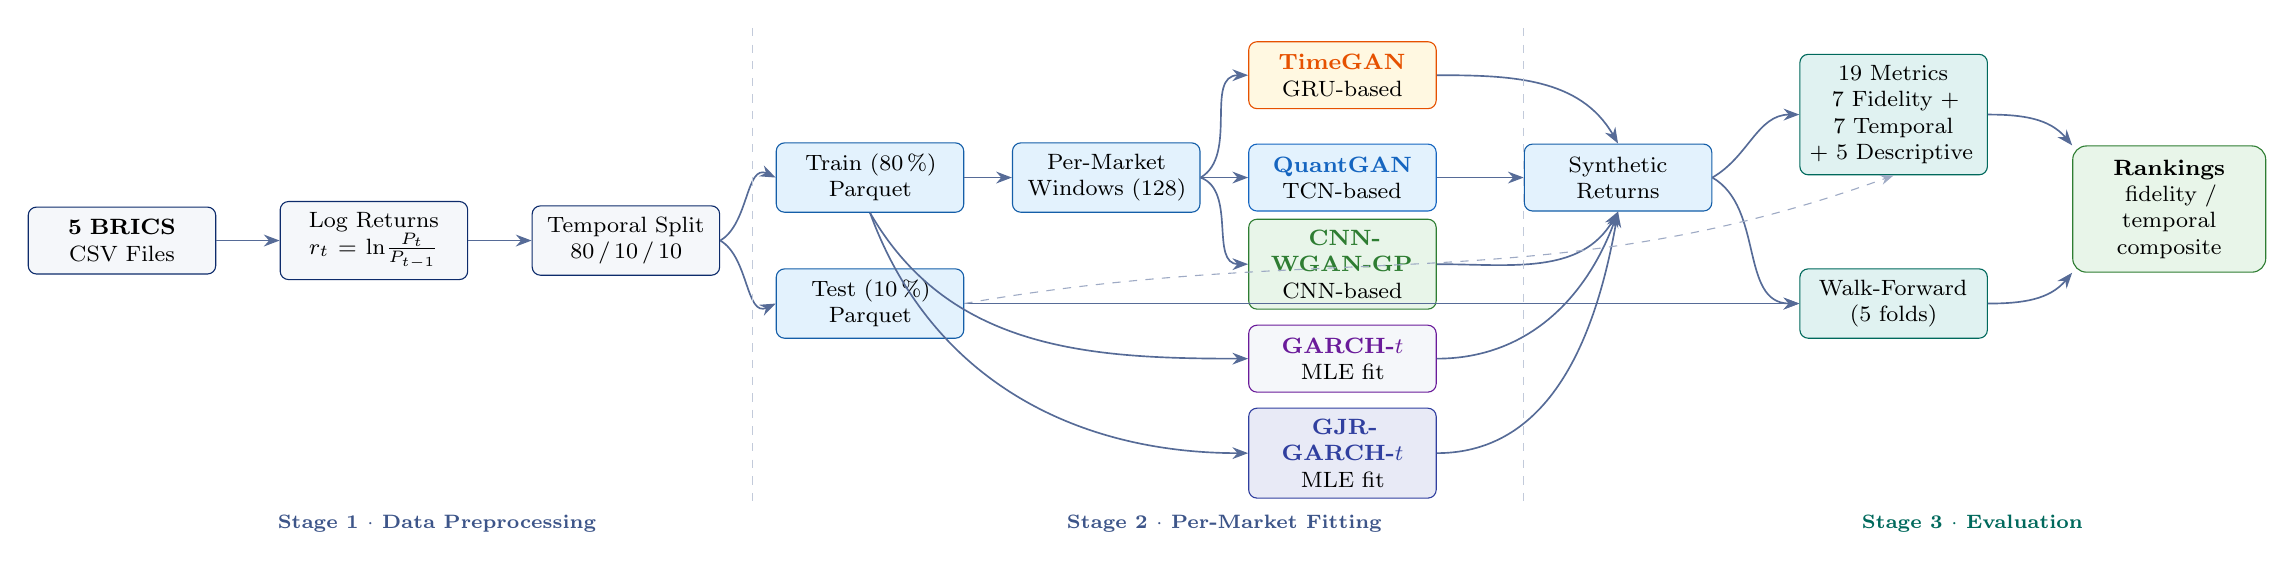
\begin{tikzpicture}[
  every node/.style={font=\footnotesize},
  pp/.style={rectangle, rounded corners=3pt, draw=Navy, fill=LBg,
             text width=2.1cm, align=center, minimum height=0.85cm, inner sep=4pt},
  sp/.style={rectangle, rounded corners=3pt, draw=Sky!80!black, fill=BBg,
             text width=2.1cm, align=center, minimum height=0.85cm, inner sep=4pt},
  ev/.style={rectangle, rounded corners=3pt, draw=Teal, fill=TealBg,
             text width=2.1cm, align=center, minimum height=0.85cm, inner sep=4pt},
  rk/.style={rectangle, rounded corners=5pt, draw=FGreen, fill=GBg,
             text width=2.1cm, align=center, minimum height=1.1cm, inner sep=5pt},
  arr/.style={-Stealth, semithick, draw=Navy!70},
  sarr/.style={-Stealth, thin, draw=Navy!40, dashed},
]
\node[pp] (csv)  at (0.0,  0.0) {\textbf{5 BRICS}\\CSV Files};
\node[pp] (lr)   at (3.2,  0.0) {Log Returns\\$r_t=\ln\!\tfrac{P_t}{P_{t-1}}$};
\node[pp] (spl)  at (6.4,  0.0) {Temporal Split\\80\,/\,10\,/\,10};
\node[sp] (trn)  at (9.5,  0.8) {Train (80\,\%)\\Parquet};
\node[sp] (tst)  at (9.5, -0.8) {Test (10\,\%)\\Parquet};
\node[sp] (poo)  at (12.5,  0.8) {Per-Market\\Windows (128)};
\node[rectangle,rounded corners=3pt,draw=TGcol,fill=ABg,
      text width=2.1cm,align=center,minimum height=0.85cm,inner sep=4pt]
     (tga) at (15.5,  2.1) {\textcolor{TGcol}{\bfseries TimeGAN}\\GRU-based};
\node[rectangle,rounded corners=3pt,draw=QGcol,fill=BBg,
      text width=2.1cm,align=center,minimum height=0.85cm,inner sep=4pt]
     (qga) at (15.5,  0.8) {\textcolor{QGcol}{\bfseries QuantGAN}\\TCN-based};
\node[rectangle,rounded corners=3pt,draw=FGcol,fill=GBg,
      text width=2.1cm,align=center,minimum height=0.85cm,inner sep=4pt]
     (fga) at (15.5, -0.3) {\textcolor{FGcol}{\bfseries CNN-WGAN-GP}\\CNN-based};
\node[rectangle,rounded corners=3pt,draw=Purple,fill=LBg,
      text width=2.1cm,align=center,minimum height=0.85cm,inner sep=4pt]
     (gar) at (15.5, -1.5) {\textcolor{Purple}{\bfseries GARCH-$t$}\\MLE fit};
\node[rectangle,rounded corners=3pt,draw=Indigo,fill=IBg,
      text width=2.1cm,align=center,minimum height=0.85cm,inner sep=4pt]
     (gjr) at (15.5, -2.7) {\textcolor{Indigo}{\bfseries GJR-GARCH-$t$}\\MLE fit};
\node[sp] (syn)  at (19.0,  0.8) {Synthetic\\Returns};
\node[ev] (sfm)  at (22.5,  1.6) {19 Metrics\\7 Fidelity + 7 Temporal\\+ 5 Descriptive};
\node[ev] (wfv)  at (22.5, -0.8) {Walk-Forward\\(5 folds)};
\node[rk] (rnk)  at (26.0,  0.4) {\textbf{Rankings}\\fidelity / temporal\\composite};
\draw[arr] (csv.east) -- (lr.west);
\draw[arr] (lr.east)  -- (spl.west);
\draw[arr] (spl.east) to[out= 30,in=155] (trn.west);
\draw[arr] (spl.east) to[out=-30,in=205] (tst.west);
\draw[arr] (trn.east) -- (poo.west);
\draw[arr] (poo.east) to[out= 30,in=180] (tga.west);
\draw[arr] (poo.east) --                 (qga.west);
\draw[arr] (poo.east) to[out=-20,in=180] (fga.west);
%% The econometric arm is fed from the raw training returns, not the
%% normalised 128-step windows: the tanh squash would compress exactly the
%% variance dynamics GARCH exists to model (Methods).
\draw[arr] (trn.south) to[out=-60,in=180] (gar.west);
\draw[arr] (trn.south) to[out=-70,in=180] (gjr.west);
\draw[arr] (tga.east) to[out=  0,in=120] (syn.north);
\draw[arr] (qga.east) --                 (syn.west);
\draw[arr] (fga.east) to[out=  0,in=240] (syn.south);
\draw[arr] (gar.east) to[out=  0,in=250] (syn.south);
\draw[arr] (gjr.east) to[out=  0,in=260] (syn.south);
\draw[arr]  (syn.east) to[out= 30,in=180] (sfm.west);
\draw[arr]  (syn.east) to[out=-30,in=180] (wfv.west);
\draw[arr]  (tst.east) --                 (wfv.west);
\draw[sarr] (tst.east) to[out=10,in=200]  (sfm.south);
\draw[arr] (sfm.east) to[out=0,in=130] (rnk.north west);
\draw[arr] (wfv.east) to[out=0,in=230] (rnk.south west);
\node[font=\scriptsize\bfseries,text=Navy!80]  at ( 4.0,-3.6) {Stage 1 $\cdot$ Data Preprocessing};
\node[font=\scriptsize\bfseries,text=Navy!80]  at (14.0,-3.6) {Stage 2 $\cdot$ Per-Market Fitting};
\node[font=\scriptsize\bfseries,text=Teal]     at (23.5,-3.6) {Stage 3 $\cdot$ Evaluation};
\draw[very thin,dashed,Navy!25] ( 8.0, 2.7) -- ( 8.0,-3.4);
\draw[very thin,dashed,Navy!25] (17.8, 2.7) -- (17.8,-3.4);
\end{tikzpicture}
}
\end{center}

\vspace{6pt}
\begin{multicols}{2}
\small

\navybox{Stage 1 --- Data Preprocessing}{%
Raw price CSVs are converted to daily log returns $r_t = \ln(P_t/P_{t-1})$. Dates are parsed and sorted chronologically. A strict temporal 80/10/10 split ensures no future data leaks into training. Files saved as Parquet for efficient I/O.}

\skybox{Stage 2 --- Per-Market Fitting (Both Families)}{%
Each 80\% training file is sliced into 128-step sliding windows for the gradient models, which normalise with z-score $+\tanh(z/3)$ and train to an asserted parity of 9,000 generator updates. The econometric models are fitted by maximum likelihood on the same market's \emph{raw} returns ($\times100$), bypassing both the windowing and the normalisation --- the $\tanh$ squash would compress the variance dynamics they exist to model. Every model is fitted \emph{independently per market}: 5 markets $\times$ 3 seeds $\times$ 5 generators, with no cross-market mixing. The shuffled control is injected alongside the model outputs at evaluation time.}

\columnbreak

\tealbox{Stage 3 --- Evaluation}{%
Generated series are compared with real test-set returns on 19 metrics: 7 Fidelity and 7 Temporal are ranked, 5 are computed and displayed but excluded from ranking (Methods). Walk-forward refits every model from scratch on 5 rolling folds. Output: fidelity\_rank, temporal\_rank, composite\_rank, and fold-level mean\,$\pm$\,sd. Downstream utility (QLIKE, Kupiec, Christoffersen) is computed per market --- see Results for the discrepancy between that and the intended pooled protocol.}

\end{multicols}

\clearpage

%% ─── ED Table 3: Architecture comparison, five models across two families ──
\pagehead{Extended Data Table 3 --- Architecture Comparison}
         {Three gradient-trained generators and two econometric baselines, side by side}

\vspace{4pt}
{\footnotesize
\setlength{\tabcolsep}{4pt}
\begin{tabularx}{\linewidth}{@{}lXXXXX@{}}
\toprule
 & \textbf{\textcolor{TGcol}{TimeGAN}} & \textbf{\textcolor{QGcol}{QuantGAN}} & \textbf{\textcolor{FGcol}{CNN-WGAN-GP}} & \textbf{\textcolor{Purple}{GARCH(1,1)-$t$}} & \textbf{\textcolor{Indigo}{GJR-GARCH-$t$}} \\
\midrule
Family & gradient & gradient & gradient & econometric & econometric \\
Core & 4-phase (embedder $+$ supervisor $+$ GAN), GRU backbone & TCN backbone, WGAN-GP & CNN deconvolution, WGAN-GP & Conditional variance, Student-$t$ innovations & GARCH $+$ leverage indicator \\
Temporal mechanism & Recurrent: each step in order, gating what to remember & Dilated causal convolutions: all time scales in one pass & Transposed convolutions: upsample noise to full sequence & $\sigma_t^2=\omega+\alpha r_{t-1}^2+\beta\sigma_{t-1}^2$ & adds $\gamma r_{t-1}^2\mathbb{1}[r_{t-1}<0]$ \\
Fitting & BCE $+$ moment matching, 4 phases & WGAN-GP, $n_\text{critic}=5$, $\lambda_\text{gp}=10$ & WGAN-GP, $n_\text{critic}=5$, $\lambda_\text{gp}=10$ & Maximum likelihood & Maximum likelihood \\
Reference & Yoon et al.\ 2019\tcite{4} & Wiese et al.\ 2020\tcite{5} & This paper; not Fin-GAN\tcite{41} & Bollerslev 1986\tcite{39} & Glosten et al.\ 1993\tcite{40} \\
Key settings & hidden\_dim 24, layers 3, lr 1e-3 & noise\_dim 100, lr 1e-4, 3 TCN blocks (dil.\ 1/2/4) & base\_channels 64, lr 1e-4, 3$\times$ConvTranspose1d & $p{=}1,q{=}1,o{=}0$, dist $t$, burn-in 500 & $p{=}1,q{=}1,o{=}1$, dist $t$, burn-in 500 \\
Input scaling & z-score $+\tanh(z/3)\to[-1,1]$ & z-score $+\tanh(z/3)\to[-1,1]$ & z-score $+\tanh(z/3)\to[-1,1]$ & Raw returns $\times100$ & Raw returns $\times100$ \\
seq\_len constraint & any & any & divisible by 8 & n/a & n/a \\
Budget & generator-update parity (asserted) & parity & parity & \textbf{exempt} --- ML fit, no step analogue & \textbf{exempt} \\
Inductive bias & Step-by-step ordering; persistence via GRU state & Multi-scale memory; dilations span short and long horizons & Coarse-to-fine hierarchical refinement, borrowed from image GANs & Conditional heteroskedasticity, symmetric response & As GARCH, plus asymmetric response to negative returns (Cont fact 5\tcite{7}) \\
\bottomrule
\end{tabularx}}

\vspace{6pt}
\pagehead{Extended Data Table 3b --- Measured Budget and Cost (This Run)}
         {From \texttt{per\_seed\_market\_performance.csv} --- econometric models are exempt, not zero}

\vspace{4pt}
{\small
\begin{tabular}{@{}llrrrc@{}}
\toprule
Model & Family & Parameters & Generator updates & Fit (s) & composite \\
\midrule
GJR-GARCH & econometric & 6 & n/a & 0.017 & 2.543 \\
GARCH & econometric & 5 & n/a & 0.018 & 2.950 \\
TimeGAN & gradient & 11,400 & 9,000 & 77.1 & 3.881 \\
FinGAN & gradient & 55,401 & 9,000 & 172.9 & 2.714 \\
QuantGAN & gradient & 276,481 & 9,000 & 464.7 & 2.912 \\
\bottomrule
\end{tabular}}

\smallskip
{\small Parameters are the trainable generator parameters for the gradient models and the fitted parameter count for the econometric ones (GARCH(1,1)-$t$: $\mu,\omega,\alpha,\beta,\nu$; GJR adds $\gamma$). \textbf{Generator updates read \texttt{n/a} for the econometric rows and this is deliberate}: a maximum-likelihood fit has no gradient-step analogue, so any number there would be fabricated, and the parity assertion the pipeline enforces is scoped to the gradient family for the same reason. Fit seconds are the mean over every (market, seed) run present. Equal generator updates is not equal compute --- QuantGAN and CNN-WGAN-GP each take $n_\text{critic}=5$ critic updates per generator update (Gulrajani et al.\ 2017\tcite{3}), and TimeGAN's \texttt{ae\_steps}/\texttt{sup\_steps} pre-training is excluded from parity and reported separately (Yoon et al.\ 2019\tcite{4}).}

\vspace{6pt}
\begin{multicols}{2}
\small

\navybox{WGAN-GP shared settings (QuantGAN \& CNN-WGAN-GP)}{%
\textbf{$n_\text{critic}=5$:} the critic must estimate the Wasserstein distance accurately before the generator uses its gradient; fewer updates leave it under-fitted and the gradient biased. Gulrajani et al.\ (2017)\tcite{3} establish this as a floor and CTBench\tcite{16} and SFAG\tcite{28} fix it identically.

\textbf{$\lambda_\text{gp}=10$:} values below 5 permit Lipschitz violations, invalidating the Kantorovich--Rubinstein duality the training objective rests on. 10 is the standard from Gulrajani et al.\ and has not been improved on.

\textbf{$\beta_1=0$ in Adam:} in adversarial training the correct generator direction reverses each time the critic updates, so momentum accumulates stale direction and pushes the wrong way. $\beta_1=0$ uses the current gradient only.

\textbf{LayerNorm, not BatchNorm, in the CNN-WGAN-GP critic:} the gradient penalty needs the critic's gradient norm at a \emph{single} interpolated point. BatchNorm makes that value depend on the other samples in the batch, corrupting the penalty.}

\columnbreak

\tealbox{TimeGAN four-phase training}{%
\textbf{Phase 1 --- autoencoder:} train embedder $e:\mathcal{X}\to\mathcal{H}$ and recovery $\hat r:\mathcal{H}\to\mathcal{X}$ on $\|X-\hat r(e(X))\|^2$.

\textbf{Phase 2 --- supervisor:} train $s:\mathcal{H}\to\hat{\mathcal{H}}$ on $\|H_{t+1}-s(H_t)\|^2$, injecting temporal causality into the latent space.

\textbf{Phase 3 --- joint adversarial:} $z\to G(z)\to s(G(z))\to\hat r(\cdot)\to\tilde X$, with
\begin{align*}
\mathcal{L}_G &= \mathcal{L}_U + 100\sqrt{\mathcal{L}_S} + 100\,\mathcal{L}_V \\
\mathcal{L}_V &= |\mu_H-\mu_{\hat H}| + |\sigma_H-\sigma_{\hat H}|
\end{align*}

\textbf{Phase 4 --- fine-tuning} of the recovery network on generated sequences.

Phases 1--2 are pre-training and are excluded from budget parity; only phase-3 joint steps are counted, matching QuantGAN's and CNN-WGAN-GP's \texttt{train\_steps}. In this run the pre-training budget was 3,000 autoencoder and 3,000 supervisor steps, reported here rather than folded into the parity figure.}

\end{multicols}

\clearpage

%% ─── ED Table 4: Metric Justifications ──────────────────────────────────────
\pagehead{Extended Data Table 4 --- Metric Justifications}
         {Definition $\cdot$ unique contribution $\cdot$ design decision $\cdot$ empirical validation $\cdot$ failure mode}

\begin{multicols}{2}
\small

\tealbox{Fidelity Group: Wasserstein and Energy Distance}{%
\textbf{Wasserstein $W_1$.} $W_1(p,q) = \inf_\gamma \E_{(x,y)\sim\gamma}\|x-y\|$ (Earth Mover's distance). Unique contribution: continuous gradient even when distributions do not overlap; stable under serial dependence. \textit{Rejected alternative:} KS $p$-value --- anti-conservative under serial correlation ($n_\text{eff} \approx n/11$ to $n/31$ for BRICS $|r|$). Empirical validation: shuffled control achieves $W_1 = 0.000\text{e+00}$ (by construction; proves KS and Wasserstein share this blind spot). Failure mode: also permutation-invariant; scores the shuffled control as perfectly matching real data.

\smallskip
\textbf{Energy distance.} $E(P,Q) = 2\E\|X-Y\| - \E\|X-X'\| - \E\|Y-Y'\|$ (Sz\'{e}kely \& Rizzo 2004\tcite{11}). Proper metric on the space of distributions; $E \geq 0$; $E=0 \Leftrightarrow P=Q$. Estimated via subsampled pairs ($n \leq 500$). Empirical validation: shuffled control = 2.97e-05 (near-zero by construction). Failure mode: permutation-invariant.}

\purplebox{Fidelity Group: Quantile MSE and Moment/Tail Diffs}{%
\textbf{Quantile MSE.} $\text{QMSE} = K^{-1}\sum_{k=1}^K [Q_\text{real}(\alpha_k) - Q_\text{syn}(\alpha_k)]^2$, $K=99$. Unique contribution: the only meaningful pointwise comparison between two unaligned distributions (compare by rank, not by index). Captures tail differences at the 1st and 99th percentiles critical for VaR. \textit{Rejected alternative:} pointwise MSE on time-indexed values --- real and synthetic are independently generated; no temporal alignment exists.

\smallskip
\textbf{Moment diffs.} mean\_diff and std\_diff are ranked within Fidelity; kurtosis\_diff and skewness\_diff are computed and displayed but never ranked (see Tail index diff below, and Methods). All four are permutation-invariant --- the shuffled control scores every one of them at the optimum --- which is part of why an unweighted mean over all metrics is won by the control.

\smallskip
\textbf{Tail index diff.} Hill estimator (Hill 1975\tcite{38}) on the top 5\% of $|r|$: $\hat{\alpha} = k/\sum \log(|r|_{(n-i)}/|r|_{(n-k)})$. This is the \emph{ranked} heavy-tail metric, because $\alpha$ exists where the fourth moment does not. \textit{Design decision:} \texttt{kurtosis\_diff} and \texttt{skewness\_diff} are computed and displayed but never ranked --- at $\hat\alpha$ 2.54--3.21 the population kurtosis is infinite in all five markets and the skewness in four, so the sample statistics diverge with $n$ rather than converging (Methods gives the measured divergence). \textit{Failure modes:} Hill sd is 0.52 at $n=995$, falling to 0.035 at $n=4{,}000$; it returns NaN above $\hat\alpha=20$ after a degenerate series once drove it to 31{,}581; and its across-run dispersion here exceeds the spread between model means (Results, Table~6), so no single-run winner on it is reported.}

\columnbreak

\purplebox{Temporal Group: ACF-MAE Triple}{%
For log-returns $r_t$, compute the sample ACF of $r_t$, $|r_t|$, and $r_t^2$ up to lag 20. Metric: mean absolute error between real and synthetic ACF vectors.

ACF(returns) MAE tests absence of linear predictability (fact 2). ACF($|r|$) and ACF($r^2$) MAE test volatility clustering (Mandelbrot 1963\tcite{9}, fact 3).

\textit{Failure mode, measured:} these metrics are ordering-sensitive by construction and do separate the econometric models from the shuffled control --- but they do \emph{not} separate the three GANs from it. Averaged over all 15 market-seeds the control scores 0.0570 on ACF$(r^2)$ MAE, beating every GAN, and only GARCH, GJR-GARCH clear it (Results, Table~3). Reported as a result about the generators, not as grounds for reclassifying the metric.

\textit{Why not ARCH-LM?} ACF-MAE is continuous with no saturation regime. ARCH-LM saturates on real data ($|\Delta p| = 0.000000$). ACF-MAE achieves 88\% MC accuracy on simulated GARCH; ARCH-LM achieves 99\% on simulated GARCH but 0\% (ratings the shuffled control as a perfect match) on real data.}

\navybox{Temporal Group: Hurst and Residual Kurtosis}{%
\textbf{Hurst exponent.} $\E[R_n/S_n] \sim c\cdot n^H$, applied to $|r_t|$ (not raw $r_t$; sign flips destroy long memory on raw returns). $H>0.5$: long memory. Metric: $|H_\text{real} - H_\text{syn}|$. Estimated by R/S (Hurst 1951\tcite{23}). Failure mode: sd 0.022 at $n=1{,}000$, 0.004 at $n=4{,}000$.

\textbf{Residual kurtosis.} Fit GARCH(1,1) by Gaussian QMLE, extract $\varepsilon_t = r_t/\sigma_t$, report excess kurtosis; reported per model as the real-vs-synthetic difference \texttt{resid\_kurtosis\_diff}. Tests fact 7 (Bollerslev 1987\tcite{36}). \textit{Design decision:} Gaussian rather than Student-$t$ QMLE, because a $t$ specification absorbs the excess kurtosis by construction and makes the test uninformative for every model. \textit{Known limitation:} two of the five generators are themselves GARCH models, so they are scored partly by their own model class. The metric asks whether tails remain heavy \emph{after} GARCH has explained what it can --- which a GARCH-$t$ generator can fail, and on the measured values neither scores better than the shuffled control on it --- but it remains an advantage of degree, and it is one of seven temporal metrics rather than the temporal result on its own (Results).}

\tealbox{Temporal Group: Discriminative AUC}{%
Logistic classifier on 20-day rolling windows. AUC = 0.5 is the optimum (indistinguishability). Ranking metric: $|\text{AUC} - 0.5|$ (not raw AUC). Empirical null: $0.506 \pm 0.084$ (15 seeds, real vs real half-splits). z-score: $(\text{AUC} - 0.506)/0.084$. Measured per model across every walk-forward fold in Results, Table~4; 3 of 5 generators sit more than 1.96 null sd from it; FinGAN, GJR-GARCH do not.

\textit{Direction bug found:} ascending rank on raw AUC put 0.30 above 0.50. Fixed by ranking on distance from chance.

\textit{Null shift from CV shuffling:} adding \texttt{shuffle=True} to cross-validation folds moves null from 0.506 to 0.584, because overlapping 20-day windows place near-duplicates in both train and test. Unshuffled CV is correct.}

\end{multicols}

\end{document}
